
\documentclass[10pt,a4paper]{article}
\usepackage{f1000_styles}

%% Default: numerical citations
% \usepackage[numbers]{natbib}

%% Uncomment this lines for superscript citations instead
% \usepackage[super]{natbib}

%% Uncomment these lines for author-year citations instead
% \usepackage[round]{natbib}
% \let\cite\citep

%% lines required to use a CSL style for references
\newlength{\cslhangindent}
\setlength{\cslhangindent}{1.5em}
\newlength{\csllabelwidth}
\setlength{\csllabelwidth}{3em}
\newlength{\cslentryspacingunit} % times entry-spacing
\setlength{\cslentryspacingunit}{\parskip}
\newenvironment{CSLReferences}[2] % #1 hanging-ident, #2 entry spacing
 {% don't indent paragraphs
  \setlength{\parindent}{0pt}
  % turn on hanging indent if param 1 is 1
  \ifodd #1
  \let\oldpar\par
  \def\par{\hangindent=\cslhangindent\oldpar}
  \fi
  % set entry spacing
  \setlength{\parskip}{#2\cslentryspacingunit}
 }%
 {}
\usepackage{calc}
\newcommand{\CSLBlock}[1]{#1\hfill\break}
\newcommand{\CSLLeftMargin}[1]{\parbox[t]{\csllabelwidth}{#1}}
\newcommand{\CSLRightInline}[1]{\parbox[t]{\linewidth - \csllabelwidth}{#1}\break}
\newcommand{\CSLIndent}[1]{\hspace{\cslhangindent}#1}

%% lines to get the code chunks working
\usepackage{color}
\usepackage{fancyvrb}
\newcommand{\VerbBar}{|}
\newcommand{\VERB}{\Verb[commandchars=\\\{\}]}
\DefineVerbatimEnvironment{Highlighting}{Verbatim}{commandchars=\\\{\}}
% Add ',fontsize=\small' for more characters per line
\newenvironment{Shaded}{}{}
\newcommand{\AlertTok}[1]{\textbf{#1}}
\newcommand{\AnnotationTok}[1]{\textit{#1}}
\newcommand{\AttributeTok}[1]{#1}
\newcommand{\BaseNTok}[1]{#1}
\newcommand{\BuiltInTok}[1]{#1}
\newcommand{\CharTok}[1]{#1}
\newcommand{\CommentTok}[1]{\textit{#1}}
\newcommand{\CommentVarTok}[1]{\textit{#1}}
\newcommand{\ConstantTok}[1]{#1}
\newcommand{\ControlFlowTok}[1]{\textbf{#1}}
\newcommand{\DataTypeTok}[1]{\underline{#1}}
\newcommand{\DecValTok}[1]{#1}
\newcommand{\DocumentationTok}[1]{\textit{#1}}
\newcommand{\ErrorTok}[1]{\textbf{#1}}
\newcommand{\ExtensionTok}[1]{#1}
\newcommand{\FloatTok}[1]{#1}
\newcommand{\FunctionTok}[1]{#1}
\newcommand{\ImportTok}[1]{#1}
\newcommand{\InformationTok}[1]{\textit{#1}}
\newcommand{\KeywordTok}[1]{\textbf{#1}}
\newcommand{\NormalTok}[1]{#1}
\newcommand{\OperatorTok}[1]{#1}
\newcommand{\OtherTok}[1]{#1}
\newcommand{\PreprocessorTok}[1]{\textbf{#1}}
\newcommand{\RegionMarkerTok}[1]{#1}
\newcommand{\SpecialCharTok}[1]{#1}
\newcommand{\SpecialStringTok}[1]{#1}
\newcommand{\StringTok}[1]{#1}
\newcommand{\VariableTok}[1]{#1}
\newcommand{\VerbatimStringTok}[1]{#1}
\newcommand{\WarningTok}[1]{\textit{#1}}

%% lines to enable bulletpoints in a new notation style
\providecommand{\tightlist}{%
  \setlength{\itemsep}{0pt}\setlength{\parskip}{0pt}}

\begin{document}
\pagestyle{fancy}

\title{Applying a Multiverse to Population Habitat Analyses}
\author[1]{Benjamin Michael Marshall*}
\author[1]{Alexander Bradley Duthie**}
\affil[1]{Biological and Environmental Sciences, Faculty of Natural Sciences, University of Stirling, Stirling, FK9 4LA, Scotland, UK}

\affil[*]{\href{mailto:benjaminmichaelmarshall@gmail.com}{\nolinkurl{benjaminmichaelmarshall@gmail.com}}}
\affil[**]{\href{mailto:alexander.duthie@stir.ac.uk}{\nolinkurl{alexander.duthie@stir.ac.uk}}}

\maketitle
\thispagestyle{fancy}

\begin{abstract}

abc

\end{abstract}

\section*{Keywords}

Movement ecology, simulation, compana, resource selection functions, step selection function, habitat preference, habitat selection, animal movement, multiverse, research choice, researcher degrees for freedom,

\clearpage
\pagestyle{fancy}

\hypertarget{introduction}{%
\section{Introduction}\label{introduction}}

abc

\hypertarget{methods}{%
\section{Methods}\label{methods}}

\begin{Shaded}
\begin{Highlighting}[]
\NormalTok{optionsCompleteList }\OtherTok{\textless{}{-}} \FunctionTok{readRDS}\NormalTok{(here}\SpecialCharTok{::}\FunctionTok{here}\NormalTok{(}\StringTok{"data"}\NormalTok{, }\StringTok{"optionsCompleteList.rds"}\NormalTok{))}
\end{Highlighting}
\end{Shaded}

\hypertarget{simulating-the-scenarios}{%
\subsection{Simulating the Scenarios}\label{simulating-the-scenarios}}

\begin{itemize}
\item
  Landscape simulation.
\item
  abmAnimalMovement settings
\end{itemize}

We used the animal movement using abmAnimalMovement v.0.1.3.0 (\protect\hyperlink{ref-abmAnimalMovement}{Marshall \& Duthie, 2022}) to simulate the movement data of an animal with a predefined (i.e., known) habitat preference.
The abmAnimalMovement package provides an agent-based approach to simulating terrestrial animal movement using raster environmental data to guie the animals decisions.
We used the NLMR v.1.1.1 package (\protect\hyperlink{ref-NLMR}{Sciaini et al., 2018}) to generate the three required resource/environmental rasters: movement resistance, foraging quality, and shelter site quality.
The abmAnimalMovement package has systems for simulating activity cycles, three separate behavioural states (differing in movement characteristics and resource prioritisation), and site fidelity.
For the purposes of this study we used one of the pre-created example pseudo-species: Badger, described in the package manuscript.
In brief, the badger is a terrestrial species occupying several shelter sites, with a 8-12 hour activity cycle with minor seasonal variation, and is subject to differing movement resistance across the landscape.

For the purposes of the analysis we simplified the landscape information into categories --akin to the sort of land-use information more frequently available to researchers of animal movement.
We focused on foraging quality because it influences the greatest amounts of movement compared to sheltering or exploratory movements.
We converted the continuous foraging quality raster into a binary, where higher quality areas (greater than 0.5) are classed as 2, and lower quality areas as 0.

We used that simulated landscape and abmAnimalMovement to simulate a population of 3, that later can be sampled from.
All individuals of this population had the same simulation settings apart from starting location.
Therefore, the variation between individuals is due to stochasticity rather than variation in the predefined habitat preference.

\hypertarget{sampling-and-analysis-options}{%
\subsection{Sampling and Analysis Options}\label{sampling-and-analysis-options}}

\begin{itemize}
\tightlist
\item
  targets construction
\end{itemize}

To manage the sampling of the population and the compounding growth of subsequent analysis decisions, we used the targets v.0.14.2 and tarchetypes v.0.7.4 R packages (\protect\hyperlink{ref-targets}{Landau, 2021a},\protect\hyperlink{ref-tarchetypes}{b}).
These packages allowed branching workflow pipeline, while keeping track of object creation thereby optimising the compute time required to explore the multiverse of analysis choice.

\hypertarget{sampling}{%
\subsubsection{Sampling}\label{sampling}}

\begin{itemize}
\item
  tracking regime
\item
  sample size
\end{itemize}

The first decision in most animal movement studies will be concerning tracking regime.
This decision is frequently dictated by more practical considerations such as anatomy and behaviour of the animal, cost of the tracking devices, and environmental factors.
Here we aimed to cover a range of tracking regimes that vary in the frequency of location fixes (1 to 0.17 points per hour), and the total duration of tracking (15 to 60 days).
We created sub-sampled datasets based on every combination of tracking frequencies and durations, provided they would result in greater than 30 data points per individual.

An important component of assessing population level habitat selection is the number of individuals included in analysis.
Therefore, we randomly generated a number of samples from our population of 3 simulated individuals.
We varied these samples sizes from 2 to 3 individuals, and ran 1 repeats for each size.
A sample never mixed tracking regimes.

\hypertarget{analysis}{%
\subsubsection{Analysis}\label{analysis}}

Building on the decisions concerning tracking regime and population sampling, our multiverse expanded dramatically by exploring four primary analysis routes.
These routes included an area based approach using Compana analysis, and three step-based approaches including averaged individual step-selection models, two-step conditional regression models, and a Poisson model.

\begin{itemize}
\tightlist
\item
  area based: compana, area method, contour, available points, space sampling, type II/III, compana test
\end{itemize}

We ran the Compana analysis (Compositional Analysis of Habitat Use) using the \emph{adehabitatHS} v.0.3.16 (\protect\hyperlink{ref-adehabitatHS}{Calenge \& Mathieu Basille, 2023}).
Compana allows for the assessment of habitat selection of multiple animals in defined habitat types; it also allows habitat selection to be estimated at different scales.
We explored two scales in the multiverse: selection within the home range (Type III), and selection within an overall population available area (Type II).
The former design (Type III) requires availability habitats to be defined on an individual-by-individual basis, while the latter (Type II) design uses a summarised population level availability.

To define availability, we created home range polygons then sampled points within, recovering the corresponding habitat at those points.
The home range (aka availability) polygons can be generated via many different processes.
We selected to explore MCP and AKDE (Minimum Convex Polygons, Autocorrelated Kernel Density Estimators).
We used the \emph{ctmm} v.0.6.1 (\protect\hyperlink{ref-ctmm}{Fleming \& Calabrese, 2023}) package for the creation of AKDEs, and the \emph{adehabitatHR} v.0.4.20 (\protect\hyperlink{ref-adehabitatHR}{Calenge \& Scott Fortmann-Roe, 2023}) package for the MCPs.
The AKDEs required the fitting of a movement model, we fit multiple models and selected the top scoring model by AIC.
For the best model we followed recommendations of , opting to run AKDEs as weighted and using (PREML???) as both these options tend to be the most robust in scenarios of lower tracking frequencies.
There are many options involved in the creation of AKDEs that could shape habitat availability and therefore estimations of selection.
We avoided a deeper exploration as the impact of the internal AKDE choices are likely smaller than those between area methods (e.g., compared to MCPs), and the AKDE creation can more guided by the underlying data.
By comparison the MCPs have very few options inpacting their creation.
Mainly MCP size varies based on the percentage of outliers excluded from the polygon area.
For all area methods we vary this percentage: 95\%, 99\%, that correspond to increasingly large areas included in the availability polygon (i.e., covering areas that are less used by the individual).
We selected these contour values as they are the most frequently used in spatial studies

Once we had created all areas for each individual, for every combination of tracking regime (duration x frequency, total regimes: 4), we created the sample/population available areas by combining all polygons.
We used this combined polygon for the type II design, where all individuals have the same availability.

We used the availability polygons to define the extent within which we sampled habitat characteristics.
The habitat characteristics were extracted from the classified landscape raster at various points.
We varied both the number of points generated (1 to 10), as well as the pattern of how they were distributed within the polygon (random or stratified).

The final decision in the area based method approach was whether the Compana analysis was tested using randomisation or in a parametric fashion.
The former uses randomisation tests to estimate the habitat selection, while the latter uses chi-squared.

\begin{itemize}
\tightlist
\item
  ssf: Model Formula (SSF or iSSF), Available Points per Step, Distribution of Step Lengths, Distribution of Turn Angles, Model Averaging Method
\item
  twoStep: Model Formula (SSF or iSSF), Available Points per Step, Distribution of Step Lengths, Distribution of Turn Angles
\item
  poisson: Model Formula (SSF or iSSF), Available Points per Step, Distribution of Step Lengths, Distribution of Turn Angles
\end{itemize}

The other analysis pathways do not rely on an available area, instead they focus on randomly generated steps that mirror the observed movement of the animal.
As such the decisions involved in running the step-selection, two-step conditional regression, and Poisson models are largely the same.

The first decision is the number of random steps generated per observed step; we ranged this from 2 to 10.
The generation of random steps is guided by two distributions, one describing the step lengths from the last observed location, and another describing the turn angle from the last observed direction of travel.
We chose to explore the impacts of different distributions.
For the step length we explored gamma and exponential distributions; for the turn angle we explored Von Mises and uniform.

All the step-based methods require the definition of a formula, where use/available is predicted by the habitat characteristics at those locations.
Model formulation opens up many possible alternative routes of analysis, but for this exploration we focus on the impacts of integrating step and turn angle interactions with habitat characteristics.
We ran two versions of all models, one with no interactions and one where both step lengths and turn angles interaction with the habitat classification.
Previous work has suggested that the integrated (i.e., model with interactions) performs better

A key component of all the population approaches is how they translate a highly structured dataset into a overall summary.
We ran individual step selection models using the amt v.0.1.7 (\protect\hyperlink{ref-amt}{Signer, Fieberg \& Avgar, 2019}) package, to explore rudimentary summary methods.
The individual step selection models need to be averaged in some manner to extract a population mean selection.
We explore two simple options for achieving this: a naive mean of the final estimates (i.e., a mean of the estimated betas), and a model average using the \emph{MuMIn} v.1.47.5 package (\protect\hyperlink{ref-MuMIn}{Bartoń, 2023}).
The \emph{MuMIn} model average approach is weighted based on AICc.
However, AICc is not directly comparable between models fitted with different datasets.
As the model formulas are identically complex and the datasets equal in data quantity, the differences in AIC are purely describing the goodness of fit to the different datasets.
Therefore, the model average provided is weighted by model fit.

The difficulties model averaging models based on different data has led to the creation of models that account for the individual variably in the model formula.
A Two-Step Conditional Regression is one such solution, where strata (time steps) and clusters (individual animals) are accounted for.
We implemented these models using the \emph{TwoStepCLogit} v.1.2.5 (\protect\hyperlink{ref-TwoStepCLogit}{Craiu et al., 2016}) package.

More recently Muff, Signer \& Fieberg (\protect\hyperlink{ref-muff_accounting_2020}{2020}) have suggested a reformulation of the step selection models to provide faster reliable estimations of population habitat selection.
The suggestion is to reformulate the model as a Poisson model, but critically with fixed .
To avoid the slow convergence of MCMC estimation, Muff, Signer \& Fieberg (\protect\hyperlink{ref-muff_accounting_2020}{2020}) make use of integrated nested Laplace approximation (INLA) to approximate Bayesian inference.
We followed the code provided by Muff, Signer \& Fieberg (\protect\hyperlink{ref-muff_accounting_2020}{2020}) and made use of \emph{INLA} v.23.4.24 (\protect\hyperlink{ref-rue_approximate_2009}{Rue, Martino \& Chopin, 2009}; \protect\hyperlink{ref-lindgren_explicit_2011}{Lindgren, Rue \& Lindström, 2011}; \protect\hyperlink{ref-martins_bayesian_2013}{Martins et al., 2013}; \protect\hyperlink{ref-rue_bayesian_2017}{Rue et al., 2017}; \protect\hyperlink{ref-kourounis_towards_2018}{Kourounis, Fuchs \& Schenk, 2018}) to run Poisson models to estimate habitat selection.

\hypertarget{assessing-the-multiverse}{%
\subsection{Assessing the multiverse}\label{assessing-the-multiverse}}

\begin{itemize}
\tightlist
\item
  spec curves
\end{itemize}

Specification curves provide an overview of the estimates of a given range of analyses.
Tighter more steep curves suggest greater agreement between all the analysis end points.
Here we also plotted the estimates against the different decisions that results in the estimates, allowing direct comparison on how the decision impacts the variation in the estimates.

\begin{itemize}
\tightlist
\item
  brm models: one per each analysis method
\end{itemize}

To better detect the impact of decisions, while accounting for the random variation stemming from the differences in individuals/samples, we ran a number of Bayesian Regression Models.
The Bayesian Regression Models aimed to describe how much of the deviation from a median answer could be explained by the various sampling and analysis decisions.
For each analysis route we ran a model that included tracking frequency, tracking duration, sample size, and all the corresponding analysis choices.
All continuous variables were scaled to help determine their relative importance to each other: (x - mean(x))/sd(x).
For the area based Compana approach the population effects included: the continuous variable contour (continuous); and the categoric predictors sampling pattern (random, stratified), test (randomisation, parametric), area method (AKDE, MCP), and design type (II, III).
For the step-based approaches they all included: model formula (integrated, non-integrated), step distribution (gamma, exponential), turn distribution (Von Mises, uniform).
The step-selection model approach also included: averaging method (naive, MuMIn average).

We ran the Bayesian Regression Models using the \emph{brms} v.2.19.0 (\protect\hyperlink{ref-brms}{Bürkner, 2021}) package.
Once complete, we checked model convergence using rhat values, acf, and trace plots.
After assessment of the model convergence measures, we modified the running parameters .

\hypertarget{results}{%
\section{Results}\label{results}}

\hypertarget{specification-curves}{%
\subsection{Specification Curves}\label{specification-curves}}

(Fig. \ref{fig:specCurveArea}).

\begin{figure}
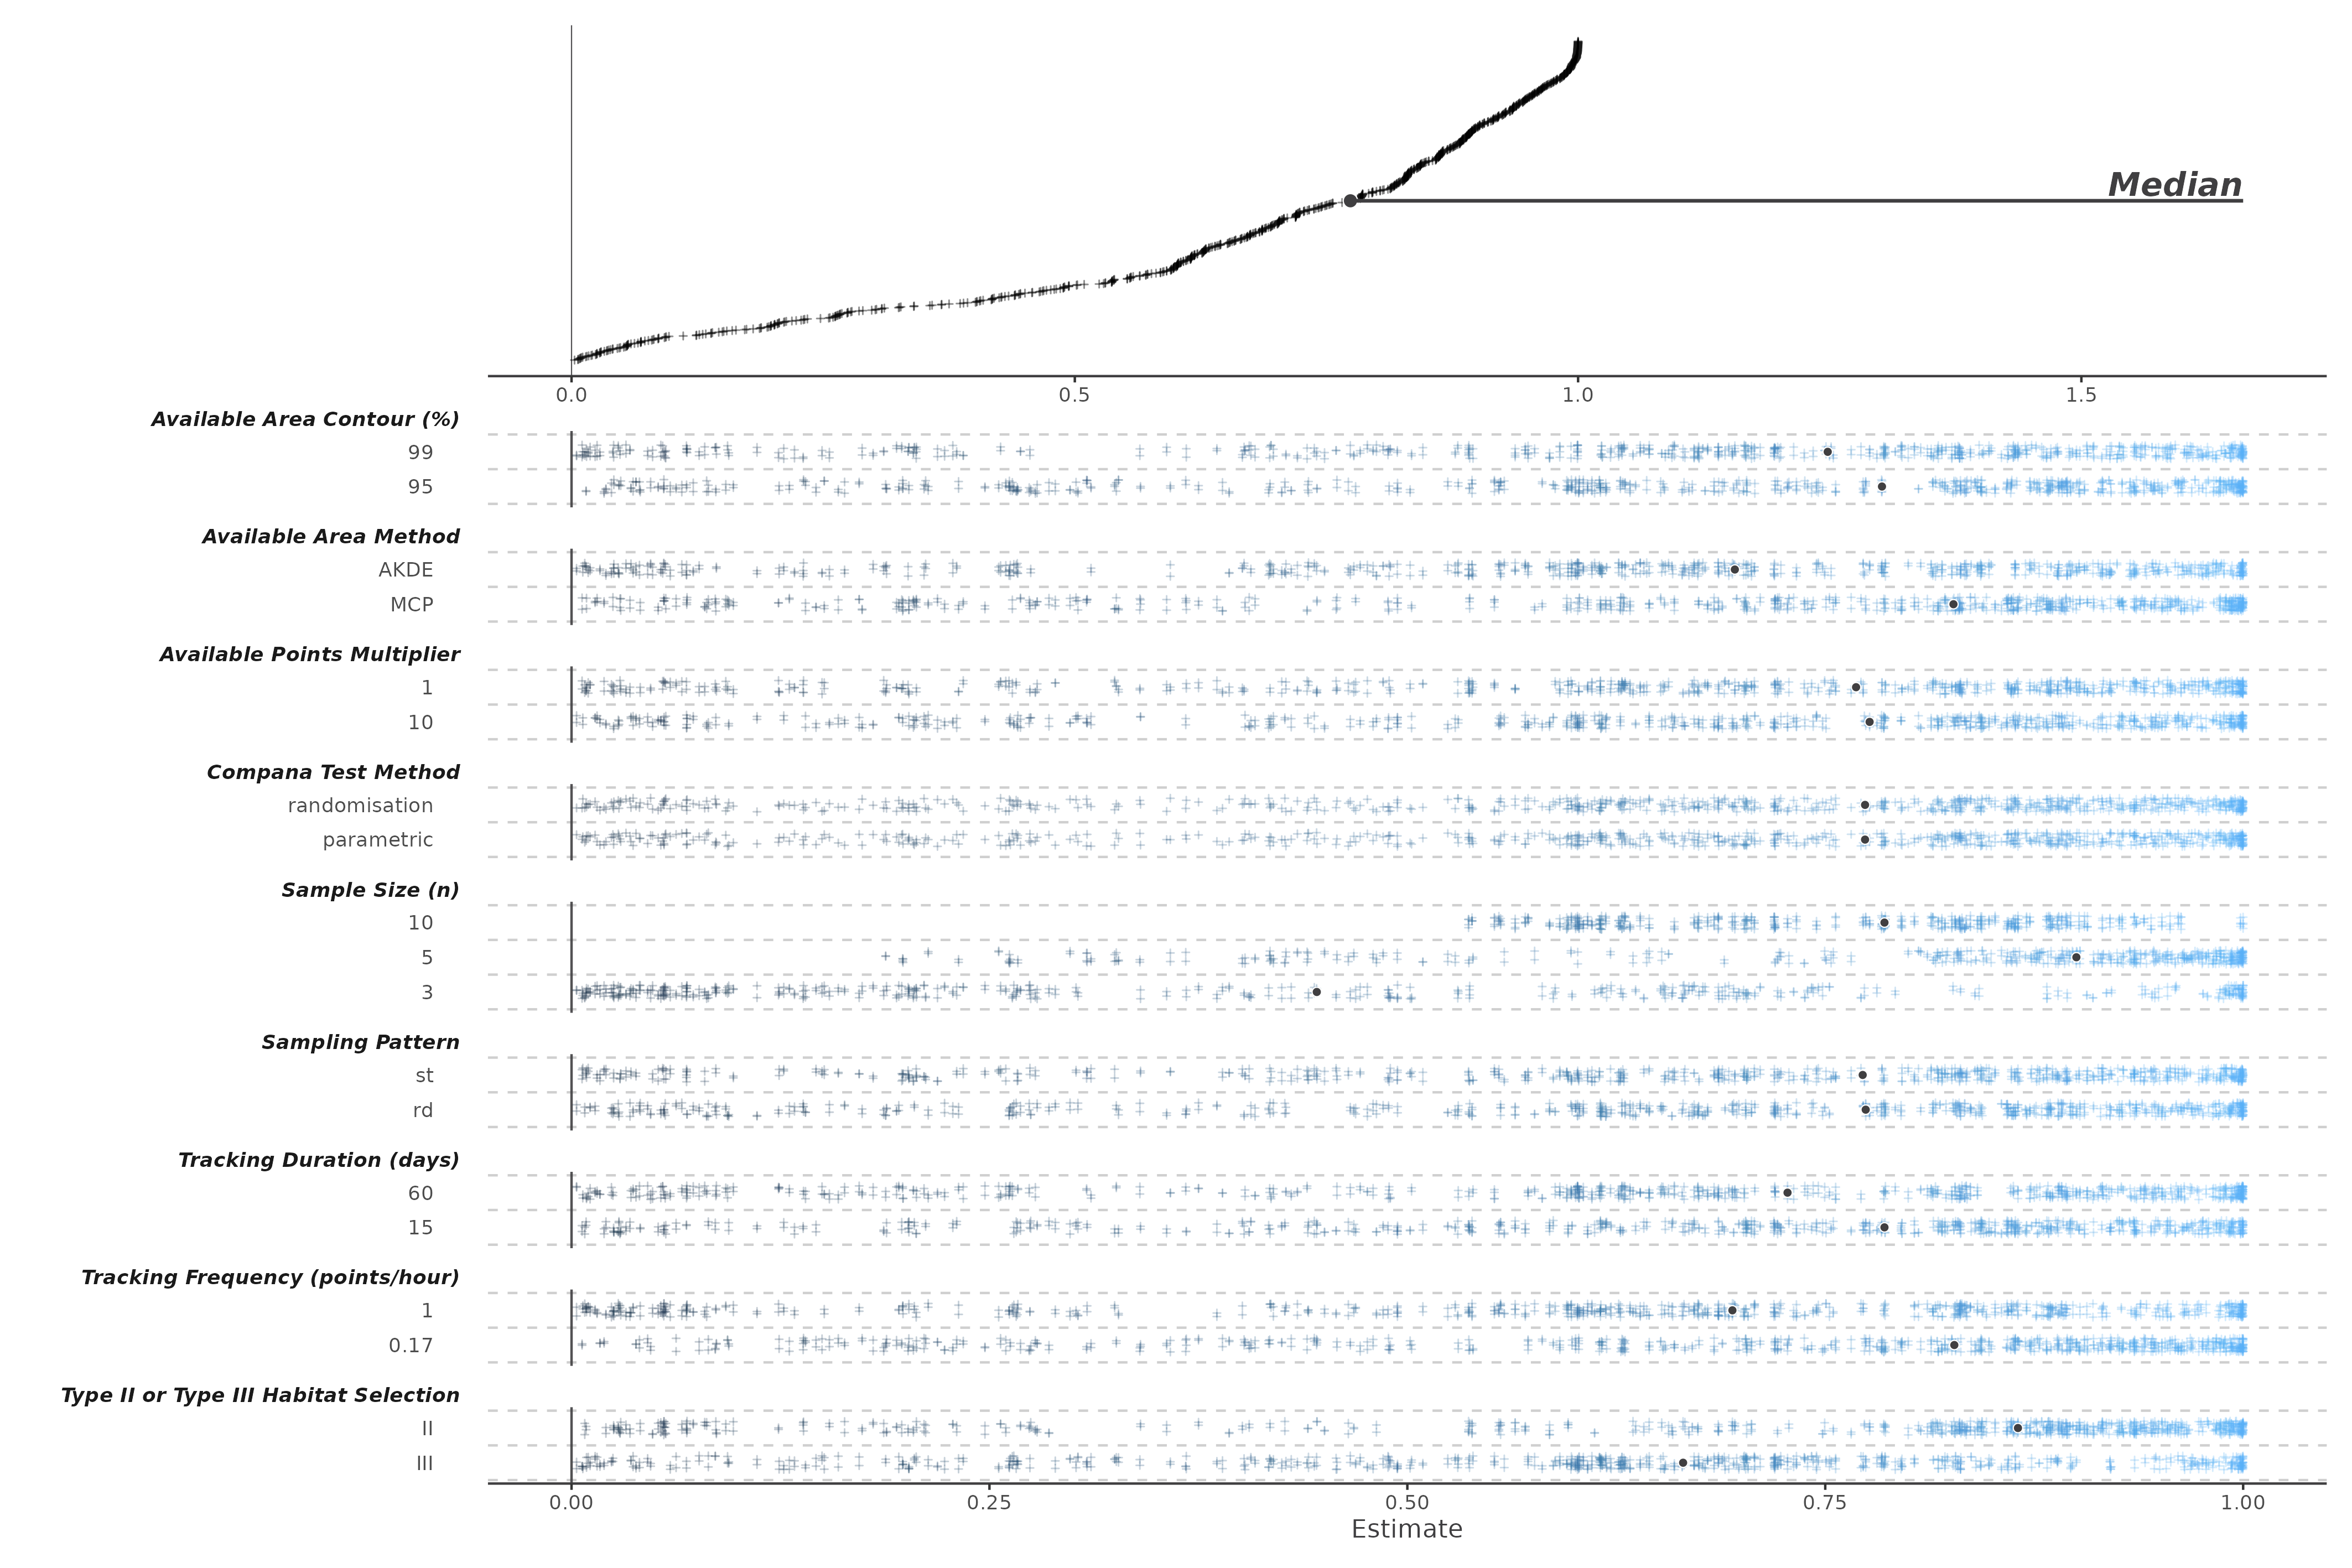
\includegraphics[width=1\linewidth]{../figures/area_specCurve} \caption{Spec curve}\label{fig:specCurveArea}
\end{figure}

(Fig. \ref{fig:specCurveSSF}).

\begin{figure}
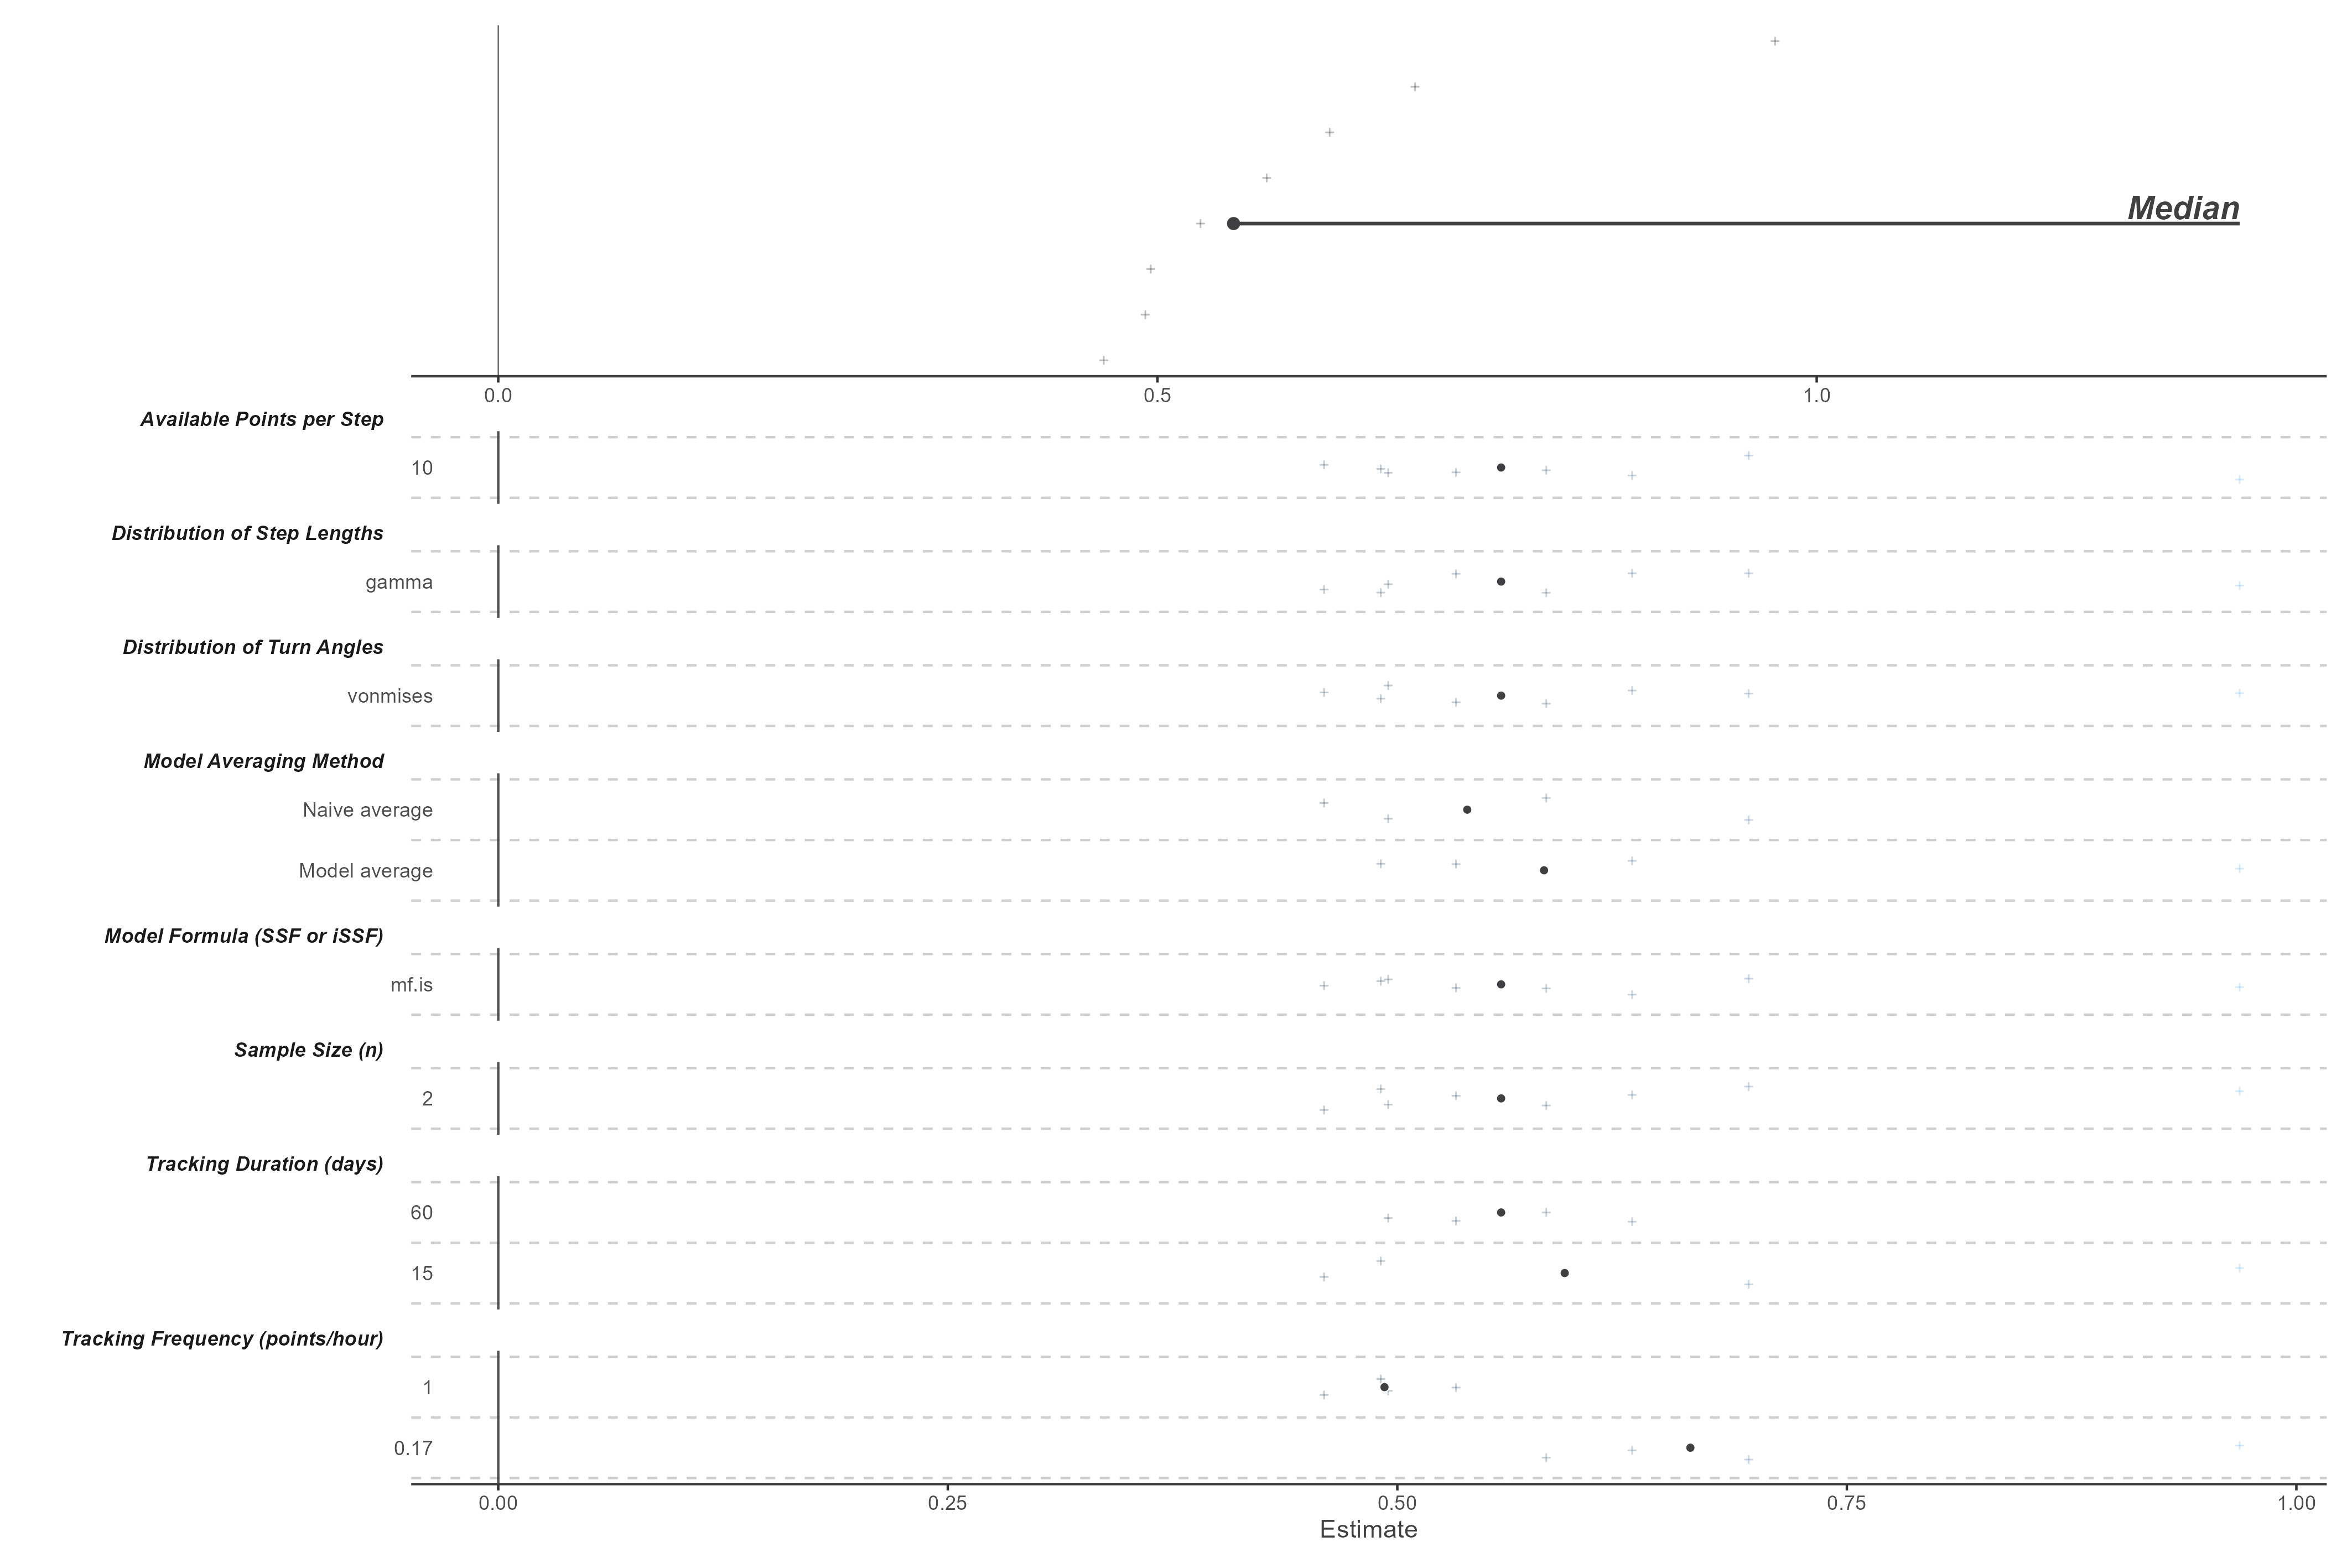
\includegraphics[width=1\linewidth]{../figures/ssf_specCurve} \caption{Spec curve}\label{fig:specCurveSSF}
\end{figure}

(Fig. \ref{fig:specCurveTwoStep}).

\begin{figure}
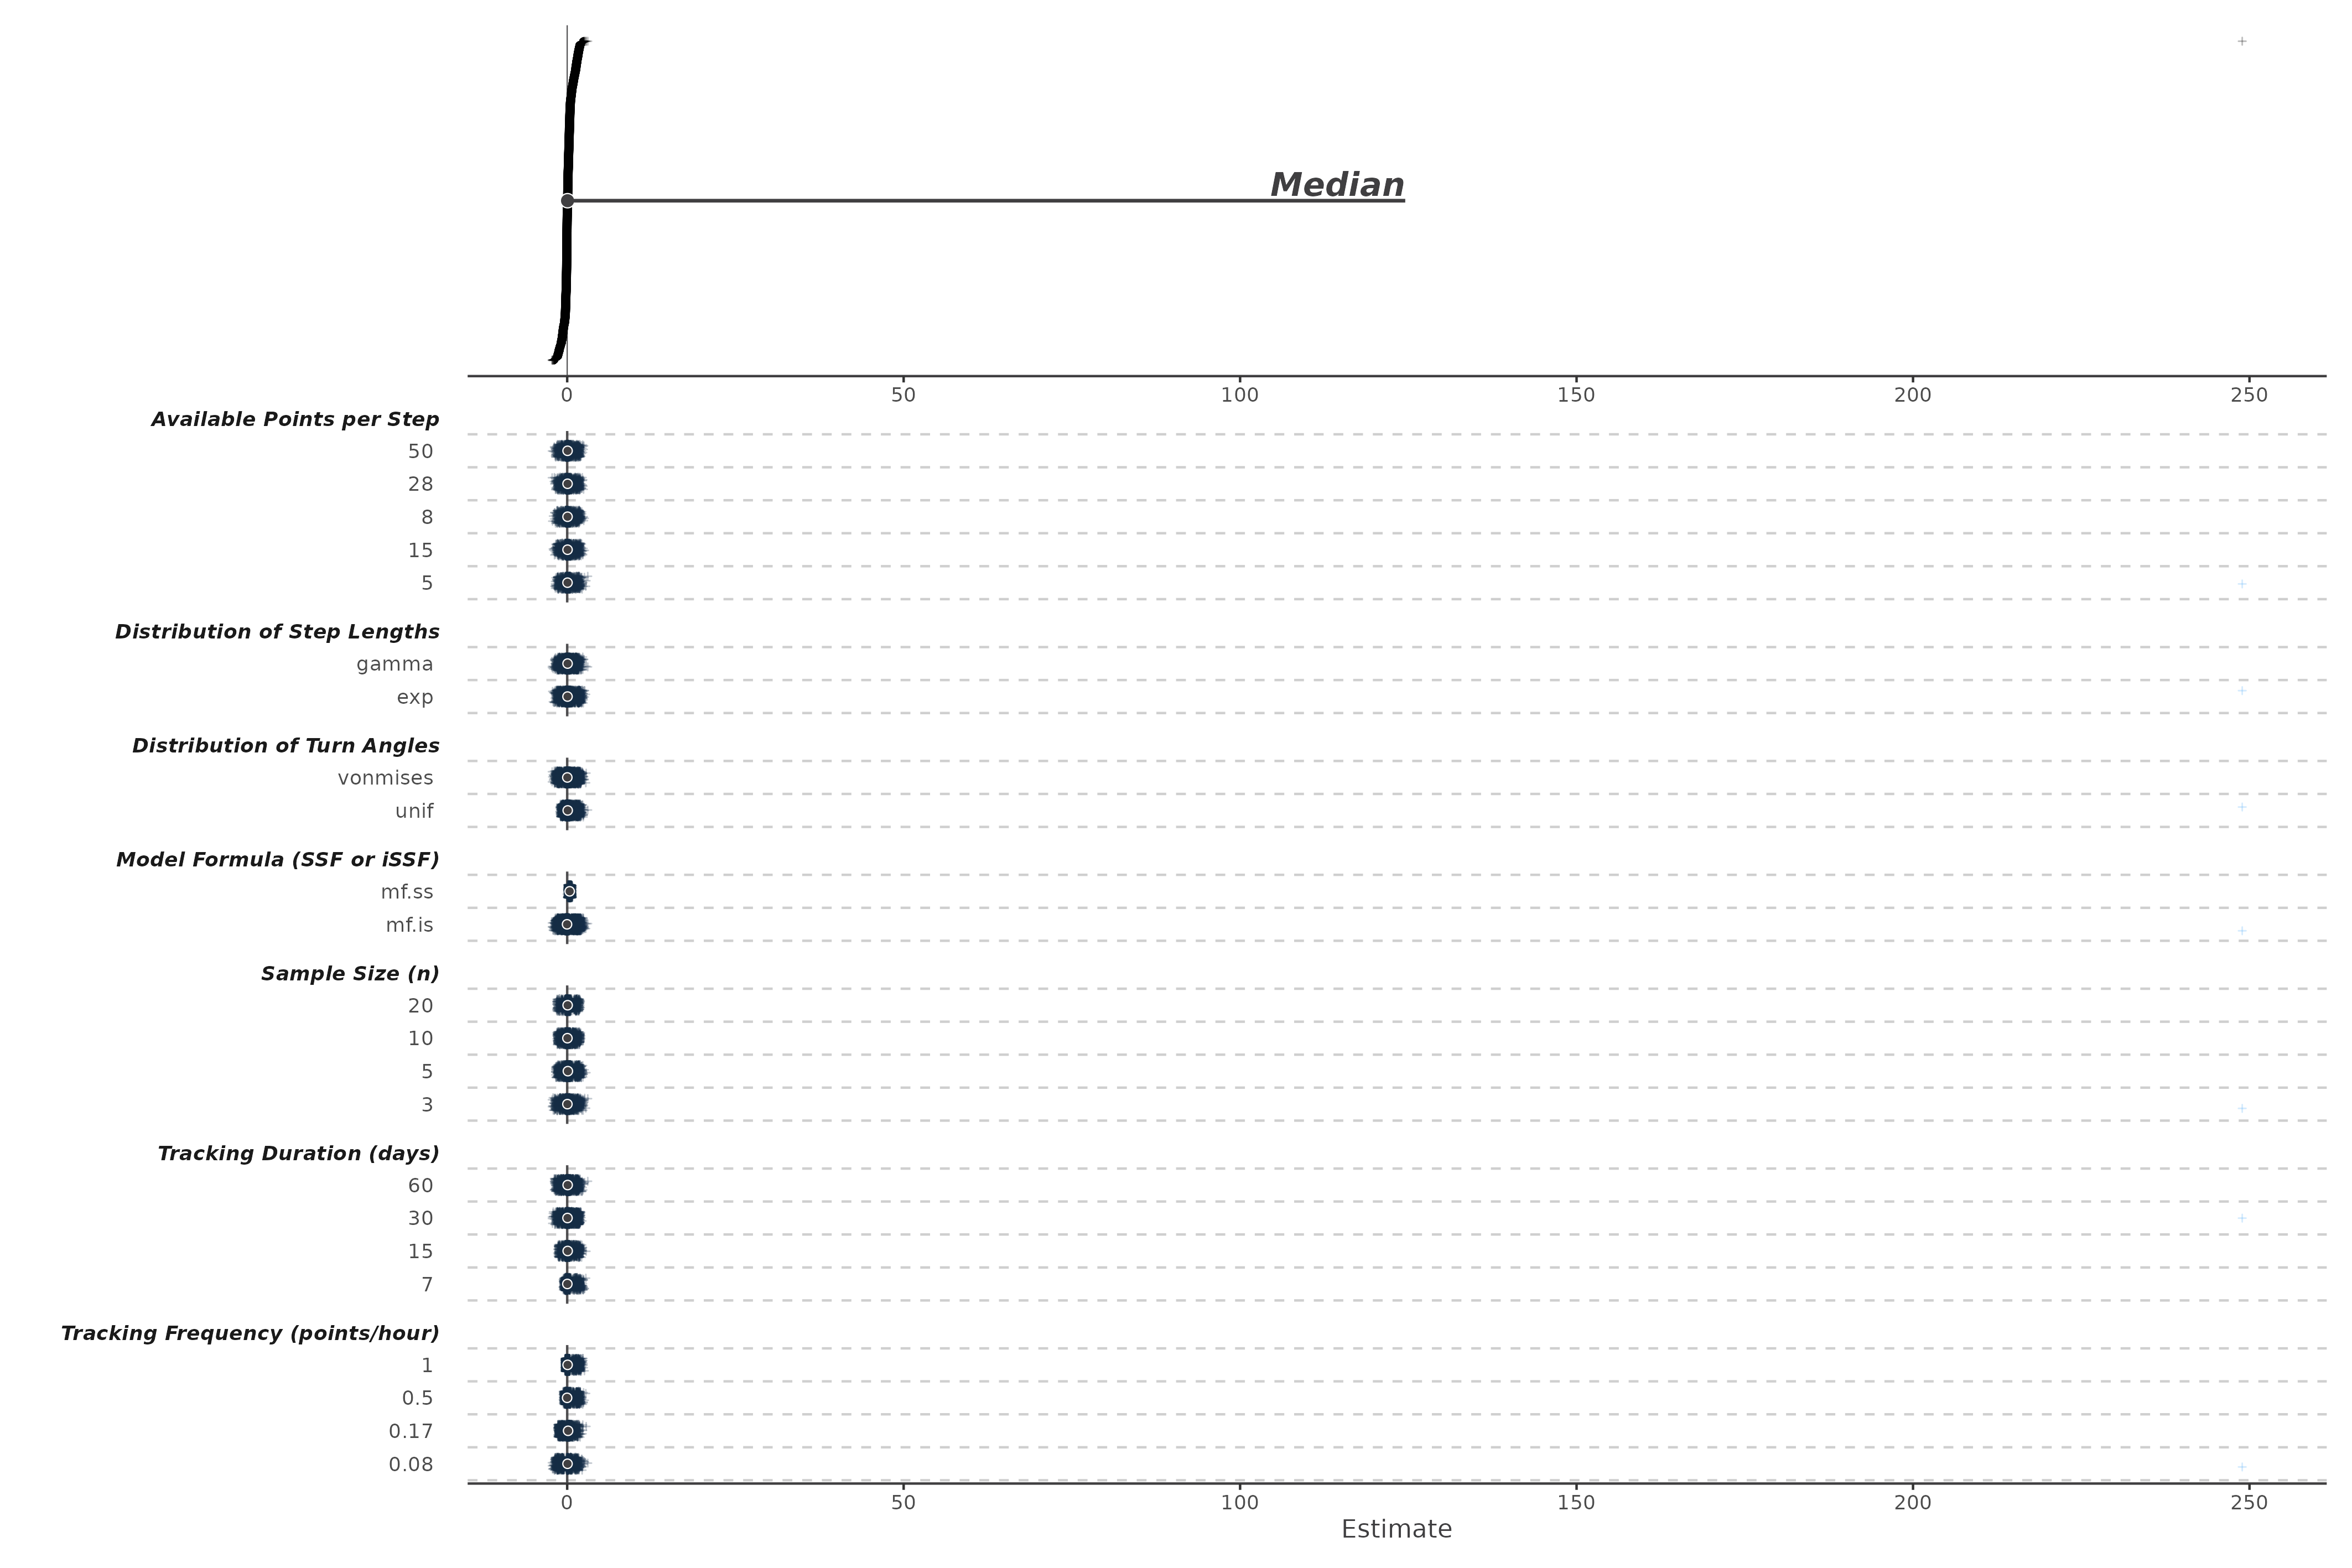
\includegraphics[width=1\linewidth]{../figures/twoStep_specCurve} \caption{Spec curve}\label{fig:specCurveTwoStep}
\end{figure}

(Fig. \ref{fig:specCurvePois}).

\begin{figure}
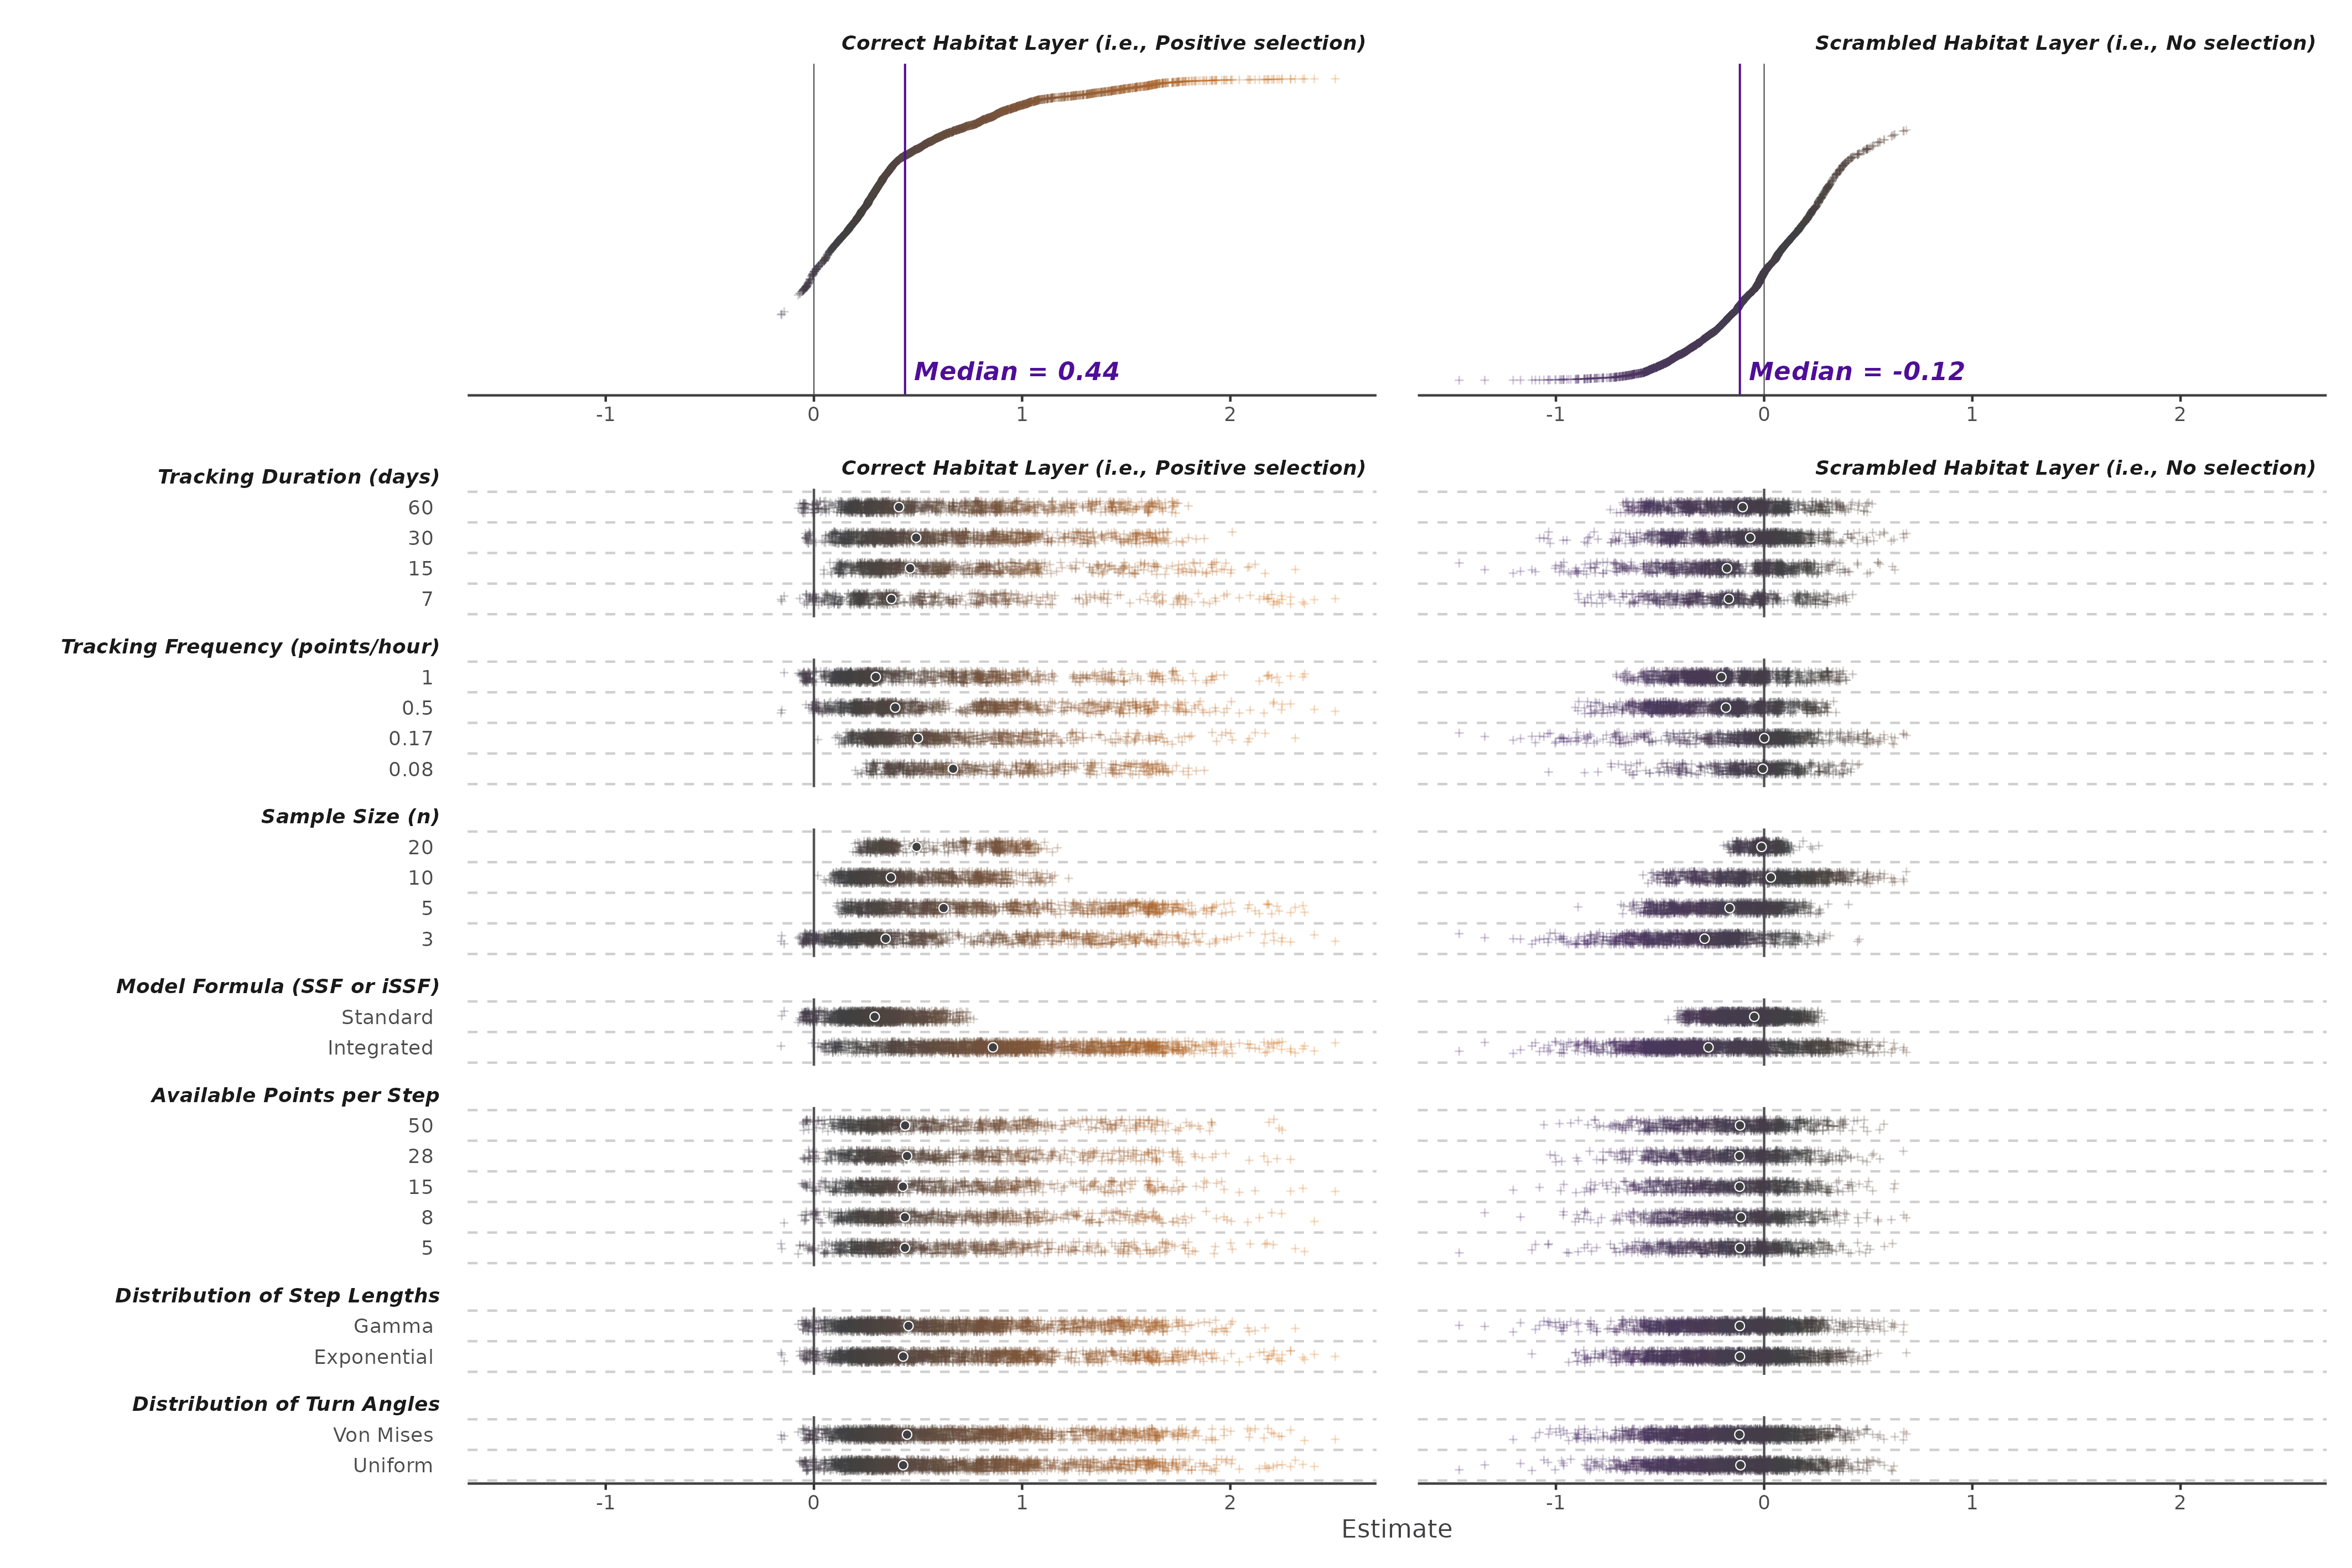
\includegraphics[width=1\linewidth]{../figures/pois_specCurve} \caption{Spec curve}\label{fig:specCurvePois}
\end{figure}

\hypertarget{model-results}{%
\subsection{Model Results}\label{model-results}}

The conditional \emph{R\textsuperscript{2}} values differed for the three models. The Compana results model had a conditional \emph{R\textsuperscript{2}} of 0.33; whereas the SSF model returned 0.59, and the Poisson model returned 0.94.

The marginal \emph{R\textsuperscript{2}} represents the bulk of the conditional \emph{R\textsuperscript{2}} suggesting an important role for the fixed/population effects. The Compana results model had a conditional \emph{R\textsuperscript{2}} of 0.48; whereas the SSF model returned 0.51, and the Poisson model returned 0.83.

The sample size was negatively correlated with deviation from the median estimate (\(\beta\) -0.03; 95\% HDCI -1.15 - 1.8).

(Fig. \ref{fig:effectPlotArea}).

\begin{figure}
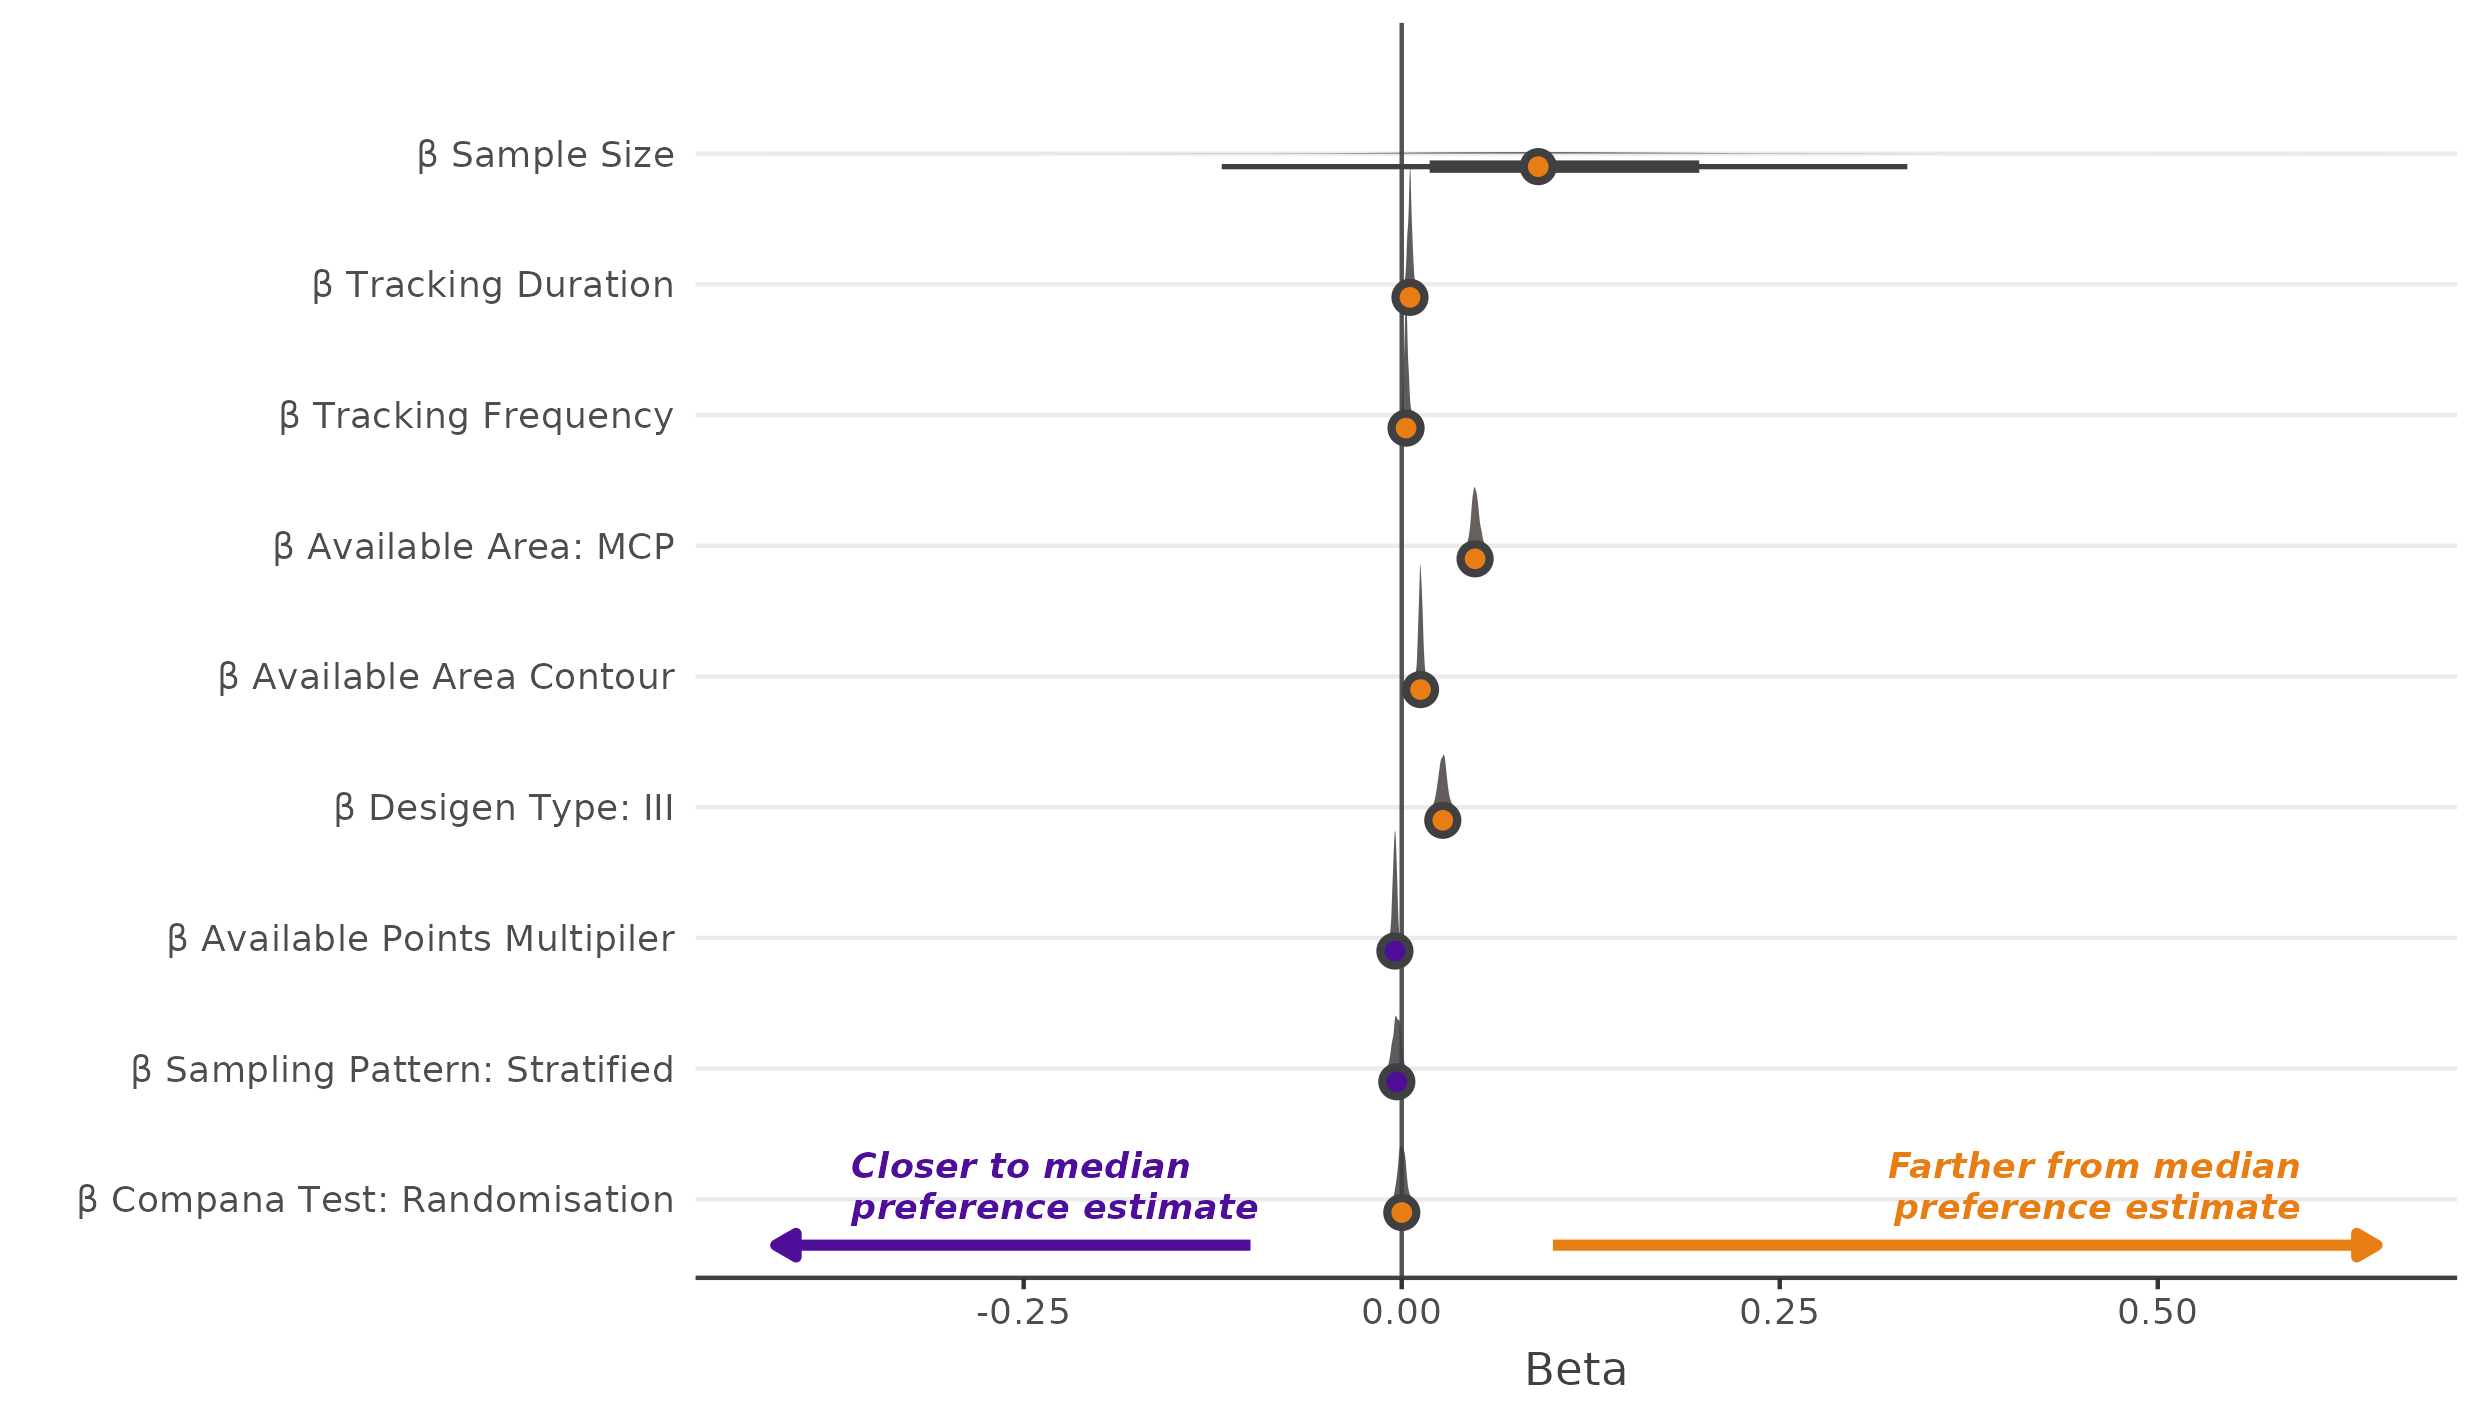
\includegraphics[width=1\linewidth]{../figures/areaBrms_effectsPlot} \caption{Beta coefs}\label{fig:effectPlotArea}
\end{figure}

(Fig. \ref{fig:effectPlotSSF}).

\begin{figure}
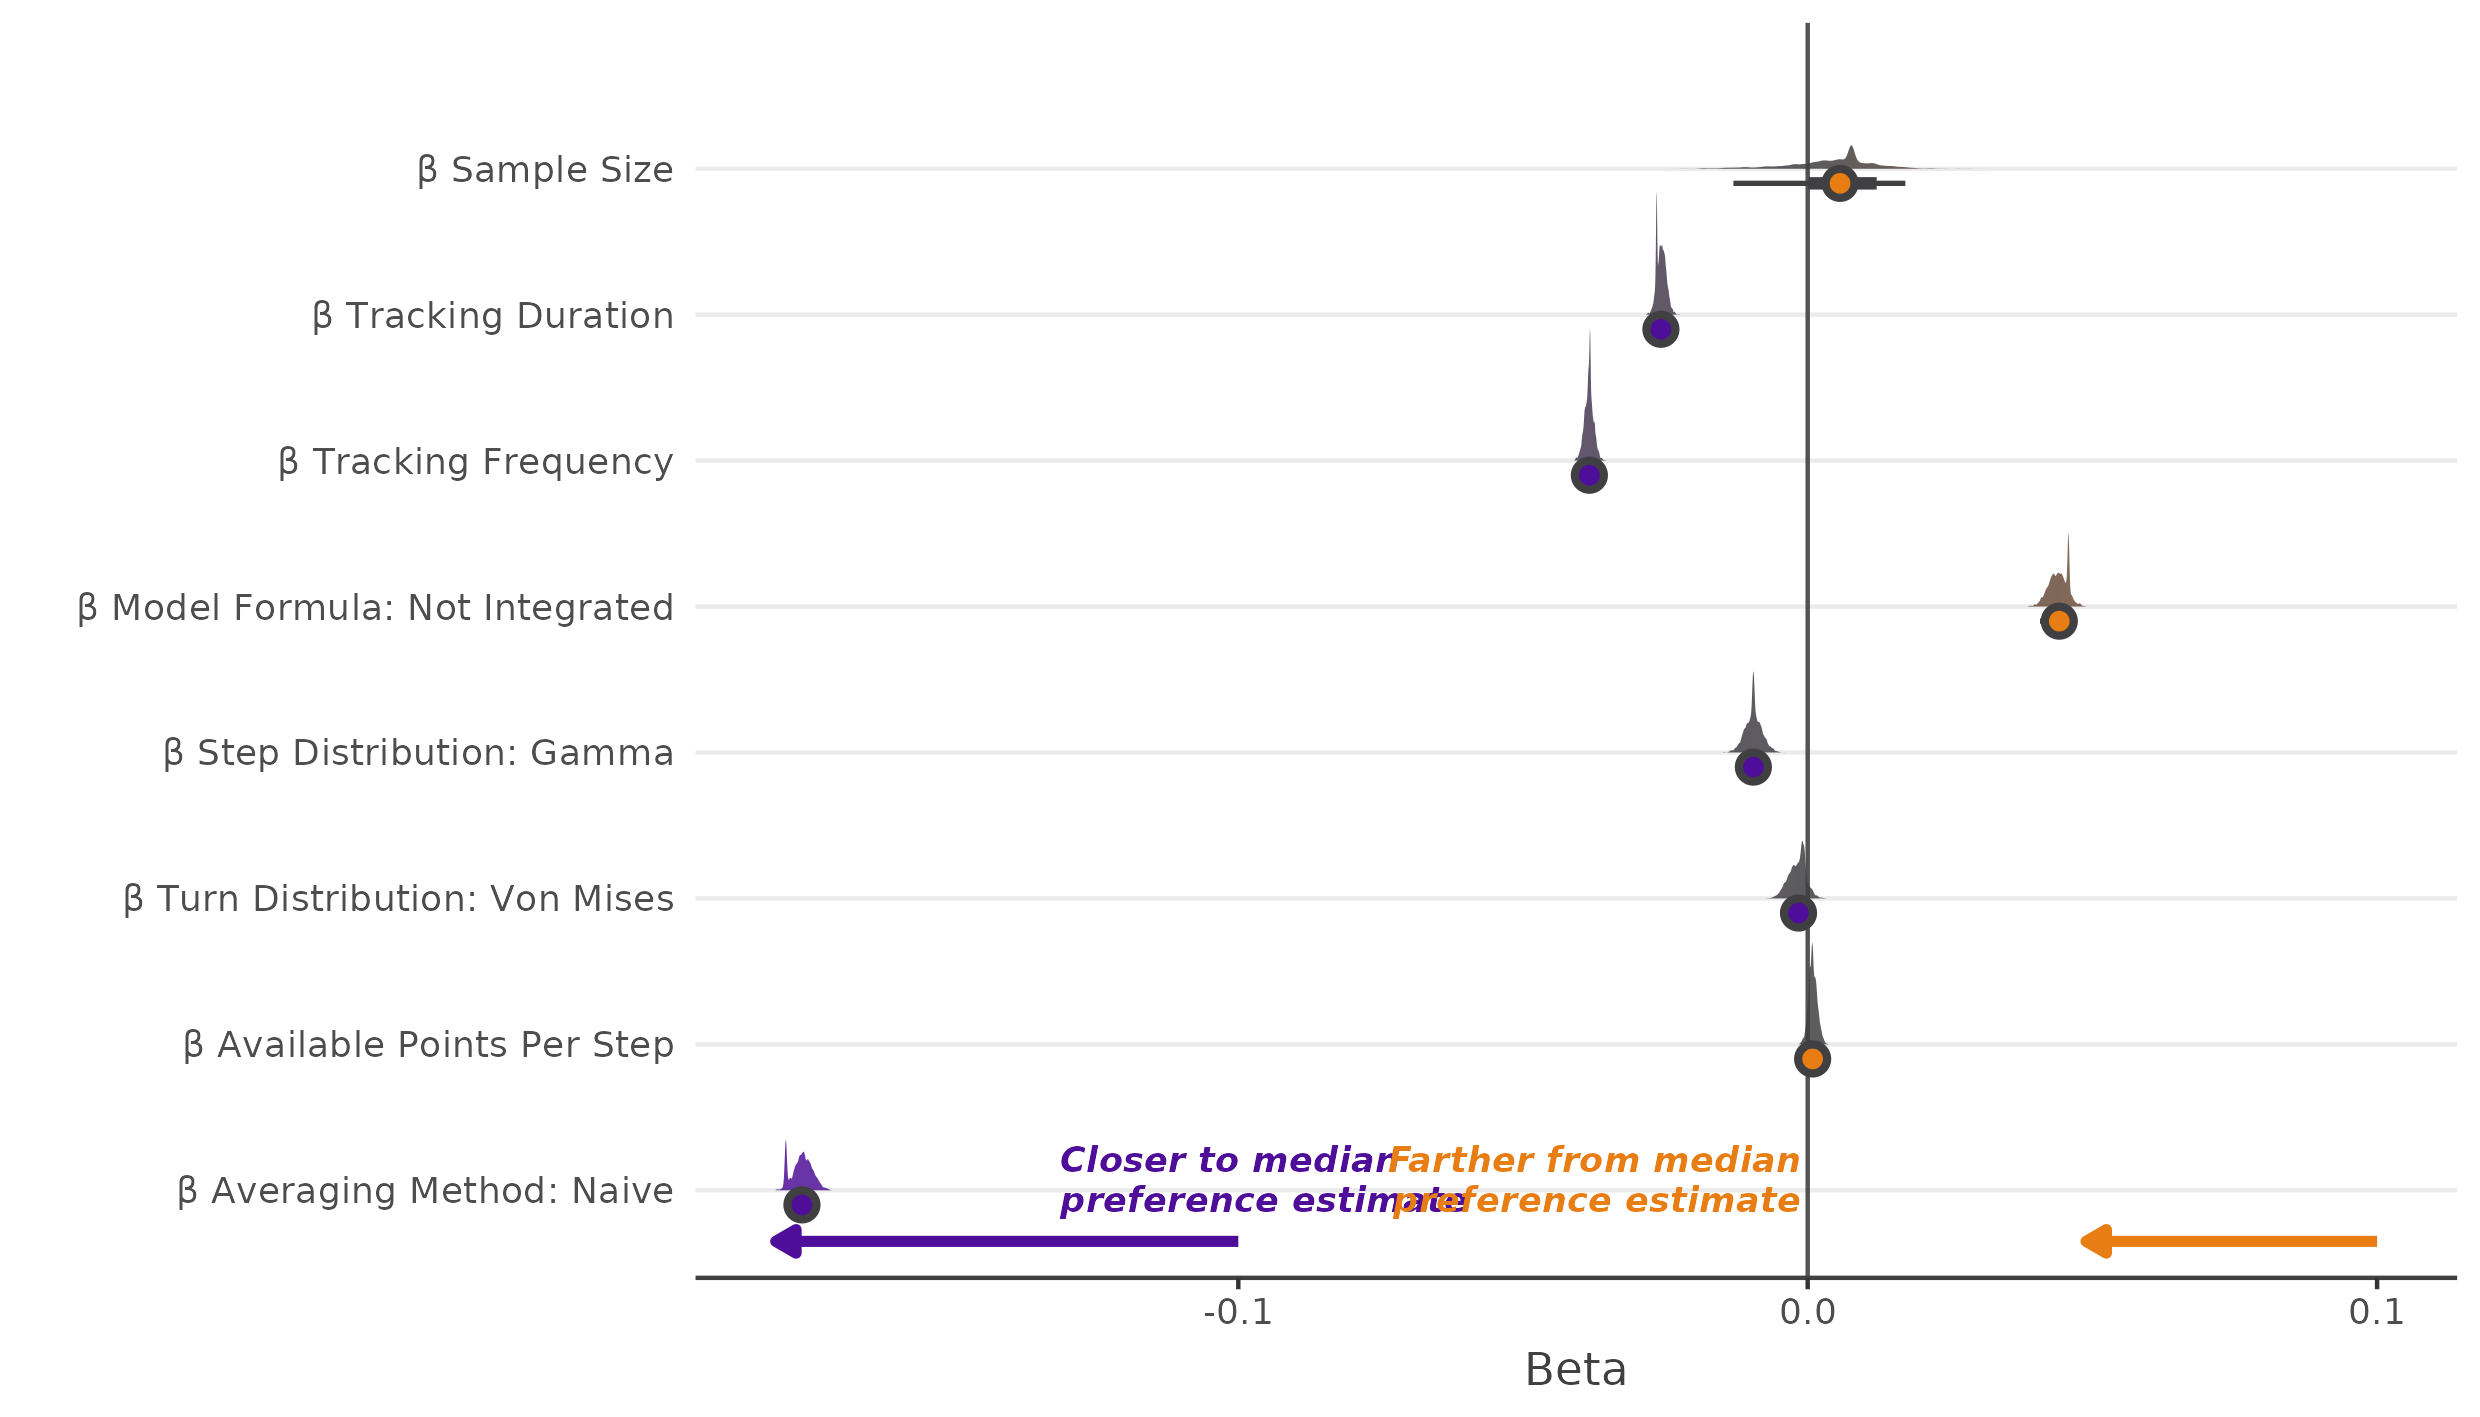
\includegraphics[width=1\linewidth]{../figures/ssfBrms_effectsPlot} \caption{Beta coefs}\label{fig:effectPlotSSF}
\end{figure}

(Fig. \ref{fig:effectPlotTwoStep}).

\begin{figure}
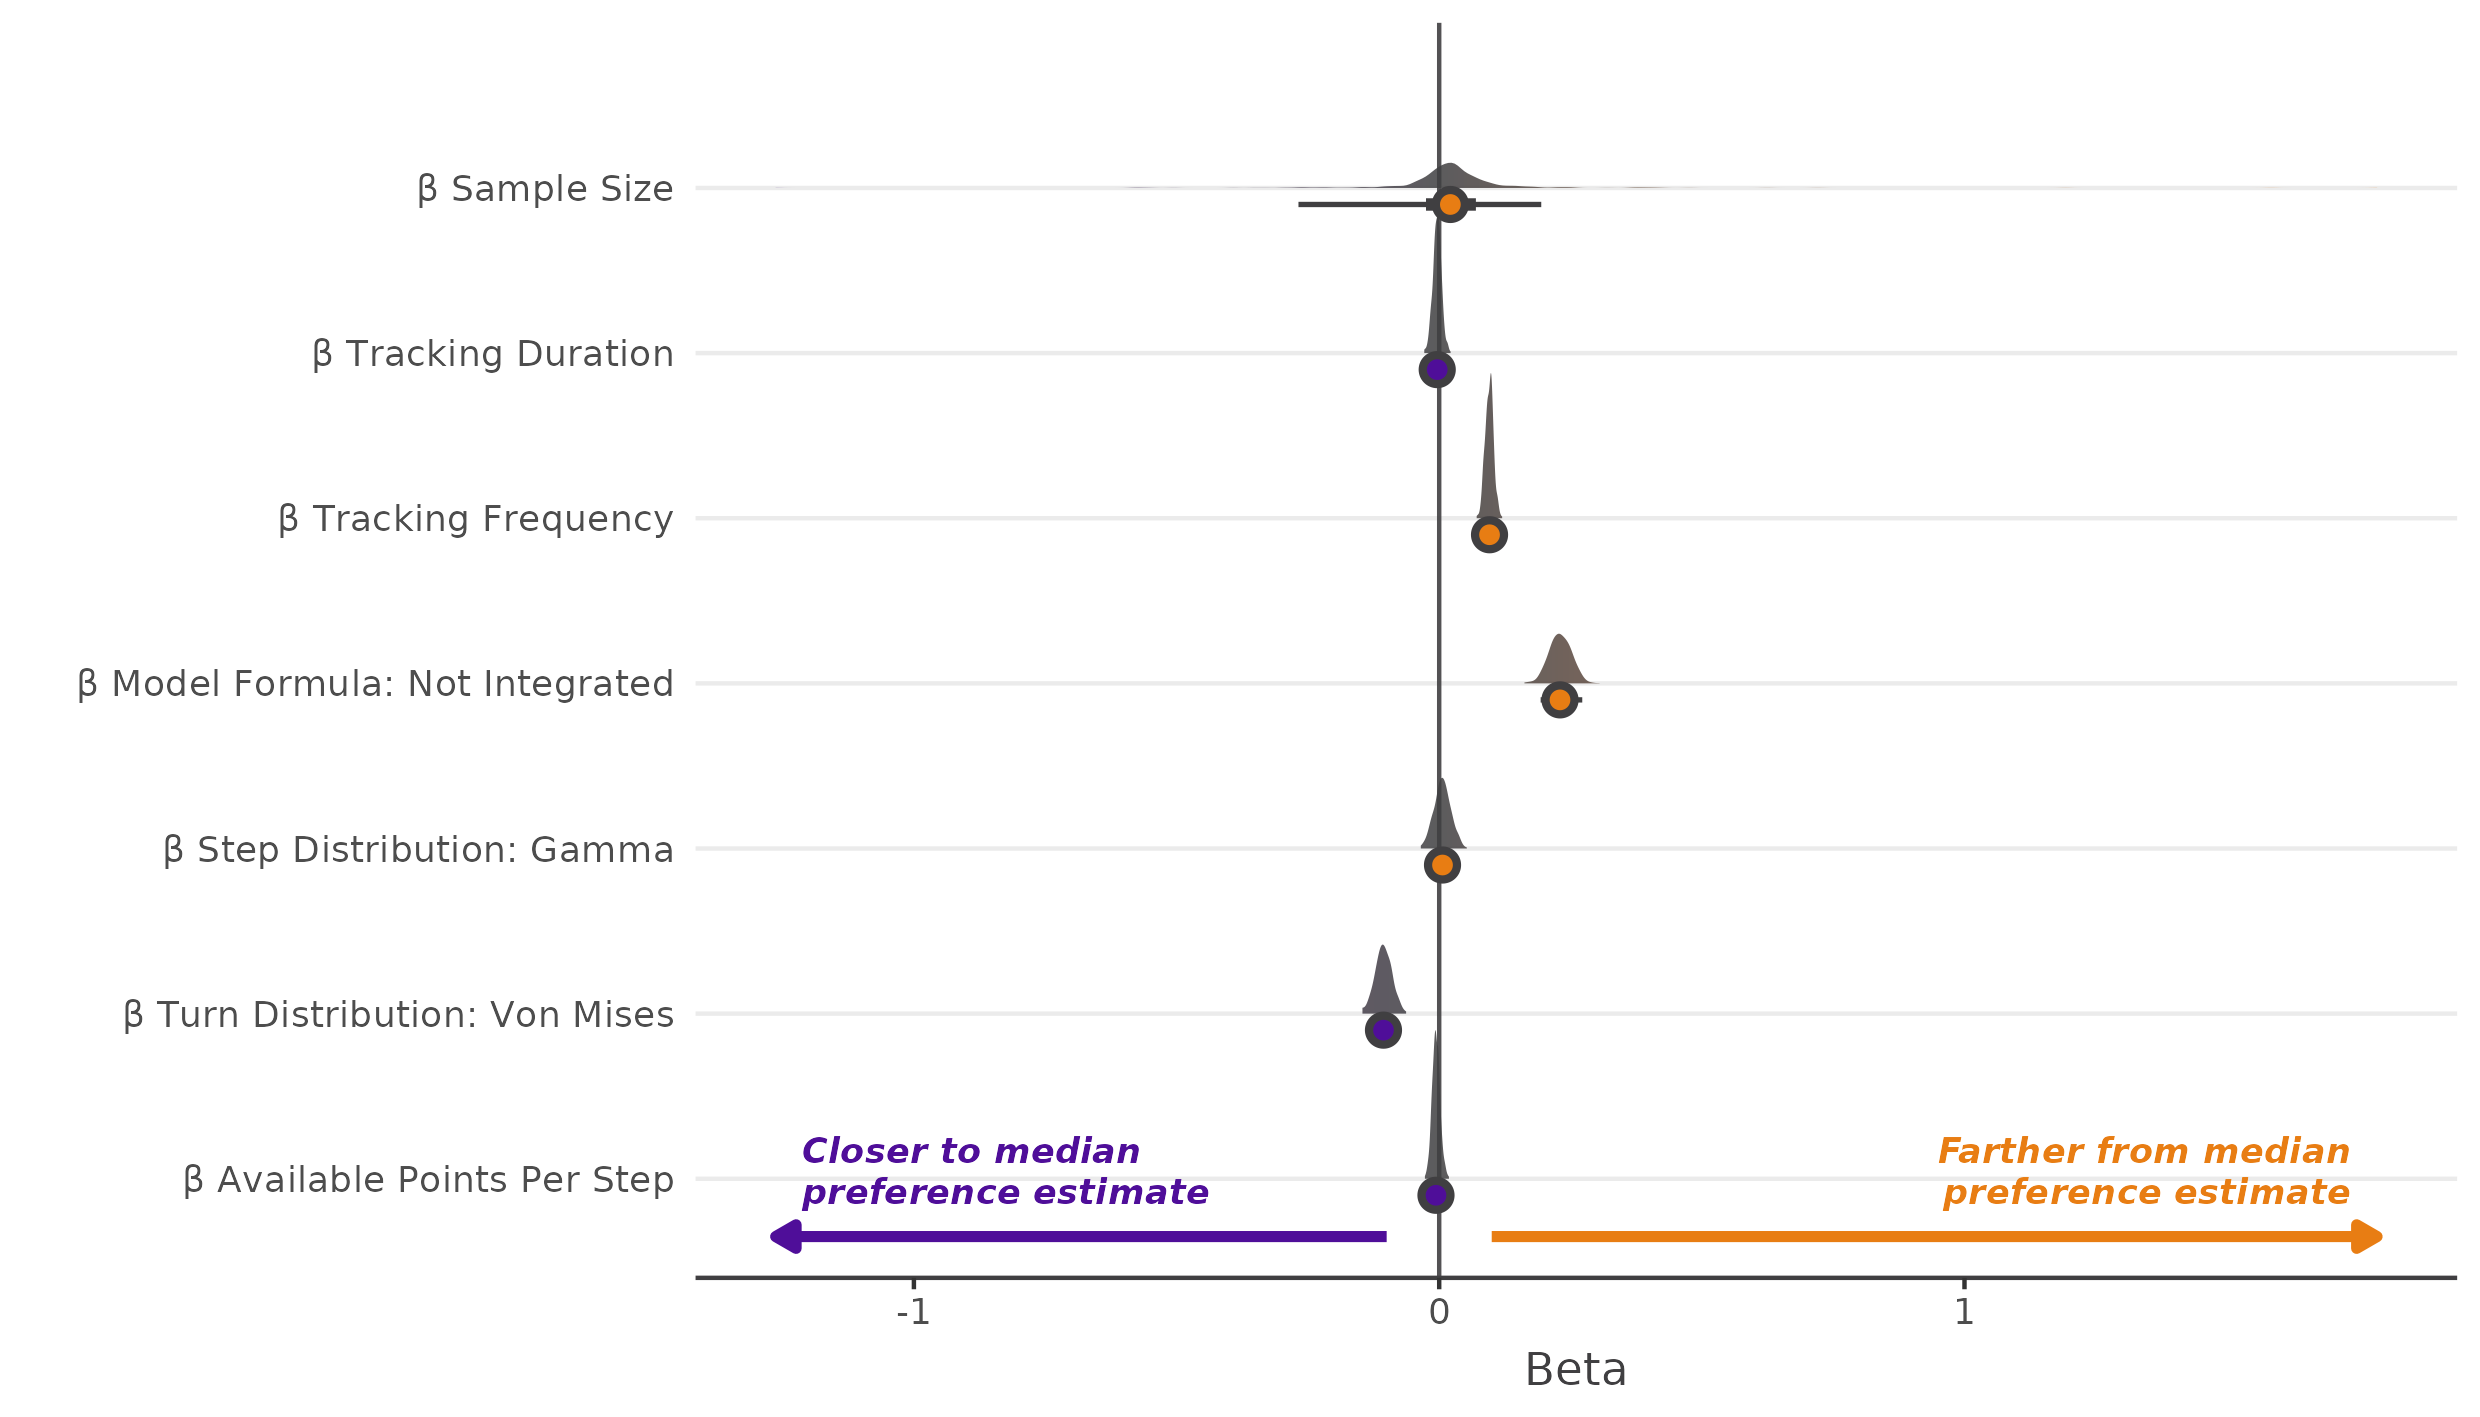
\includegraphics[width=1\linewidth]{../figures/twoStepBrms_effectsPlot} \caption{Beta coefs}\label{fig:effectPlotTwoStep}
\end{figure}

(Fig. \ref{fig:effectPlotPois}).

\begin{figure}
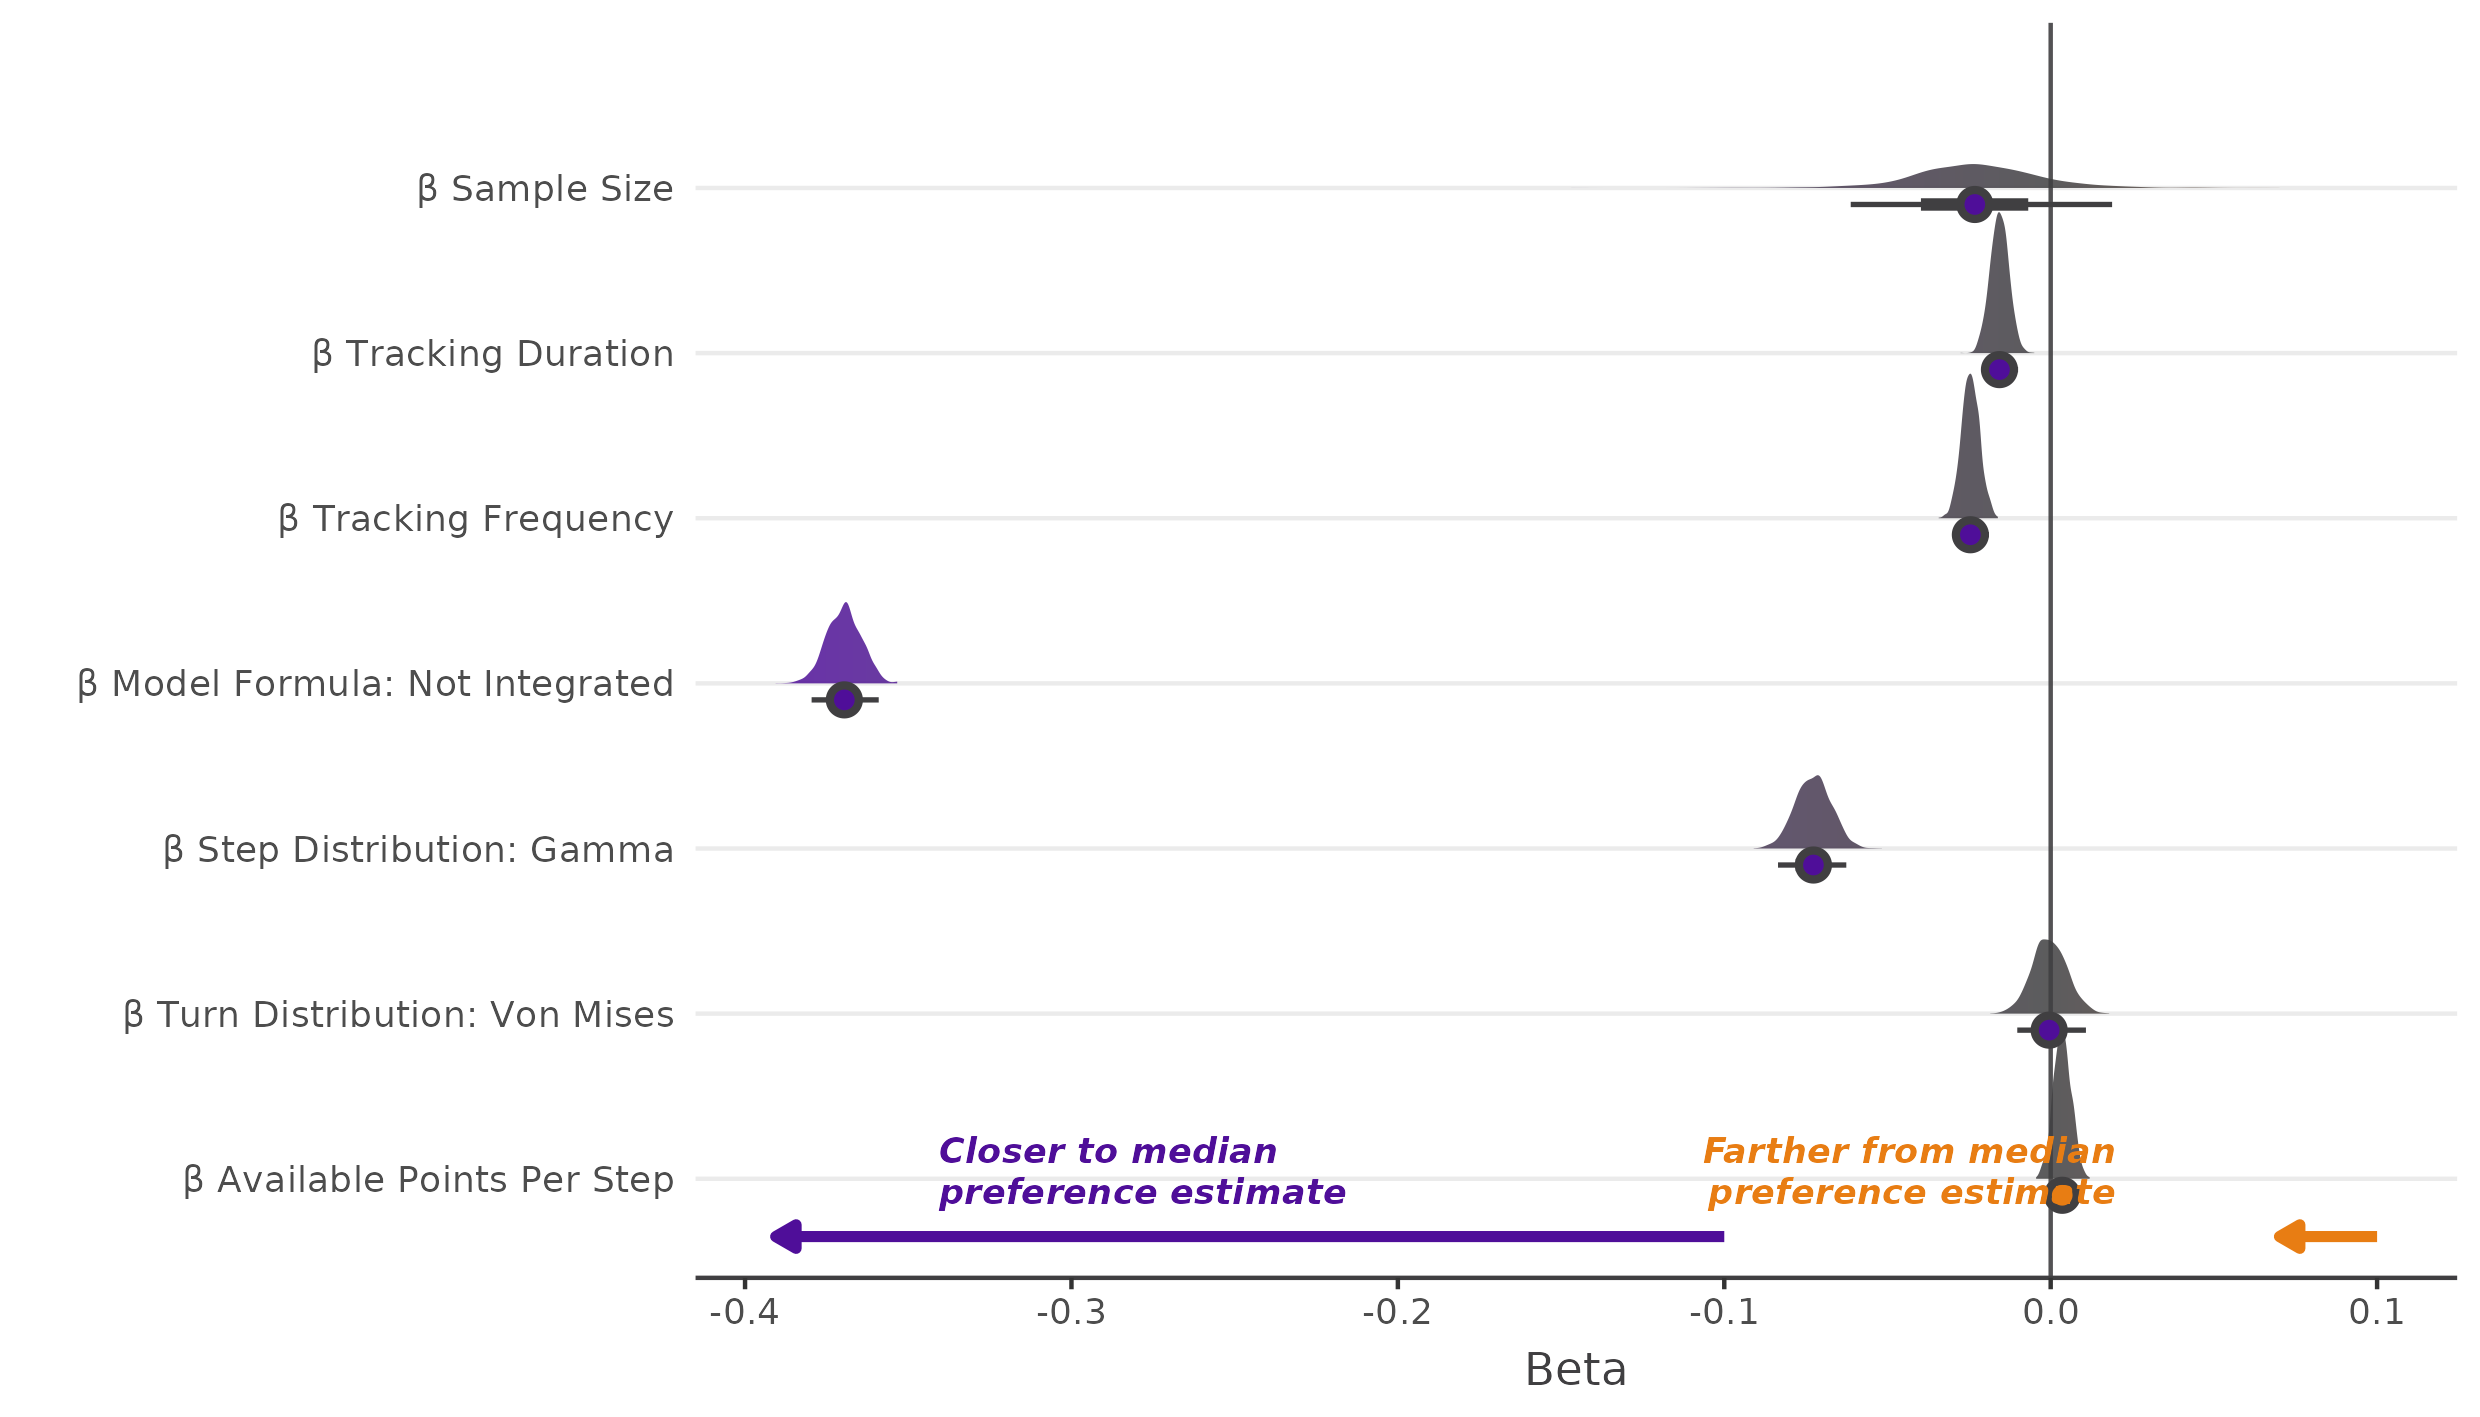
\includegraphics[width=1\linewidth]{../figures/poisBrms_effectsPlot} \caption{Beta coefs}\label{fig:effectPlotPois}
\end{figure}

\hypertarget{discussion}{%
\section{Discussion}\label{discussion}}

\hypertarget{limitations}{%
\subsection{Limitations}\label{limitations}}

\hypertarget{conclusions}{%
\subsection{Conclusions}\label{conclusions}}

\hypertarget{acknowledgements}{%
\section{Acknowledgements}\label{acknowledgements}}

BMM was funded by the Natural Environment Research Council (NERC) via the IAPETUS2 Doctoral Training Partnership.

\hypertarget{software-availablity}{%
\section{Software availablity}\label{software-availablity}}

In addition to packages already mentioned in the methods we also used the following.

We used \emph{R} v.4.2.2 (\protect\hyperlink{ref-base}{R Core Team, 2023}) via \emph{RStudio} v.2023.6.2.561 (\protect\hyperlink{ref-rstudio}{RStudio Team, 2022}).
We used \emph{here} v.1.0.1 (\protect\hyperlink{ref-here}{Müller, 2020}) and \emph{qs} v.0.25.5 (\protect\hyperlink{ref-qs}{Ching, 2023}) to manage directory addresses and saved objects.

We used \emph{raster} v.3.6.14 (\protect\hyperlink{ref-raster}{Hijmans, 2023}) and \emph{RandomFields} v.3.3.14 (\protect\hyperlink{ref-RandomFields}{Schlather et al., 2015}) to aid landscape raster creation alongside NLMR v.1.1.1 (\protect\hyperlink{ref-NLMR}{Sciaini et al., 2018}).

We used \emph{ggplot2} v.3.4.2 for creating figures (\protect\hyperlink{ref-ggplot2}{Wickham, 2016}), with the expansions: \emph{patchwork} v.1.1.2 (\protect\hyperlink{ref-patchwork}{Pedersen, 2022}), \emph{ggridges} v.0.5.4 (\protect\hyperlink{ref-ggridges}{Wilke, 2022}), and \emph{ggdist} v.3.2.0 (\protect\hyperlink{ref-ggdist}{Kay, 2023a}).

We used \emph{brms} v.2.19.0 (\protect\hyperlink{ref-brms}{Bürkner, 2021}) to run Bayesian models, with diagnostics generated used \emph{bayesplot} v.1.10.0 (\protect\hyperlink{ref-bayesplot}{Gabry et al., 2019}), \emph{tidybayes} v.3.0.2 (\protect\hyperlink{ref-tidybayes}{Kay, 2023b}), and \emph{performance} v.0.10.2 (\protect\hyperlink{ref-performance}{Lüdecke et al., 2021}).

We used the \emph{dplyr} v.1.0.10 (\protect\hyperlink{ref-dplyr}{Wickham et al., 2023}), \emph{tibble} v.3.1.8 (\protect\hyperlink{ref-tibble}{Müller \& Wickham, 2023}),
and \emph{stringr} v.1.5.0 (\protect\hyperlink{ref-stringr}{Wickham, 2022}) packages for data manipulation.

We used \emph{sp} v.1.5.1 (\protect\hyperlink{ref-sp}{Bivand, Pebesma \& Gomez-Rubio, 2013}), \emph{move} v.4.1.12 (\protect\hyperlink{ref-move}{Kranstauber, Smolla \& Scharf, 2023}) for manipulation of spatial data and estimation of space use not otherwise mentioned in the methods.

We used rmarkdown v.2.19 (\protect\hyperlink{ref-rmarkdown2018}{Xie, Allaire \& Grolemund, 2018}; \protect\hyperlink{ref-rmarkdown2020}{Xie, Dervieux \& Riederer, 2020}; \protect\hyperlink{ref-rmarkdown2023}{Allaire et al., 2023}), bookdown v.0.33 (\protect\hyperlink{ref-bookdown2016}{Xie, 2016}, \protect\hyperlink{ref-R-bookdown}{2022}), tinytex v.0.44 (\protect\hyperlink{ref-tinytex2019}{Xie, 2019}, \protect\hyperlink{ref-tinytex2023}{2023a}), and knitr v.1.41 (\protect\hyperlink{ref-knitr2014}{Xie, 2014}, \protect\hyperlink{ref-knitr2015}{2015}, \protect\hyperlink{ref-knitr2023}{2023b}) packages to generate type-set outputs.

We generated R package citations with the aid of \emph{grateful} v.0.1.13 (\protect\hyperlink{ref-grateful}{Francisco Rodríguez-Sánchez, Connor P. Jackson \& Shaurita D. Hutchins, 2023}).

\hypertarget{data-availabilty}{%
\section{Data availabilty}\label{data-availabilty}}

\hypertarget{supplementary-material}{%
\section{Supplementary Material}\label{supplementary-material}}

\hypertarget{references}{%
\section*{References}\label{references}}
\addcontentsline{toc}{section}{References}

\hypertarget{refs}{}
\begin{CSLReferences}{1}{0}
\leavevmode\vadjust pre{\hypertarget{ref-rmarkdown2023}{}}%
Allaire J, Xie Y, Dervieux C, McPherson J, Luraschi J, Ushey K, Atkins A, Wickham H, Cheng J, Chang W, Iannone R. 2023. \emph{\href{https://github.com/rstudio/rmarkdown}{{rmarkdown}: Dynamic documents for r}}.

\leavevmode\vadjust pre{\hypertarget{ref-MuMIn}{}}%
Bartoń K. 2023. \emph{\href{https://CRAN.R-project.org/package=MuMIn}{MuMIn: Multi-model inference}}.

\leavevmode\vadjust pre{\hypertarget{ref-sp}{}}%
Bivand RS, Pebesma E, Gomez-Rubio V. 2013. \emph{\href{https://asdar-book.org/}{Applied spatial data analysis with {R}, second edition}}. Springer, NY.

\leavevmode\vadjust pre{\hypertarget{ref-brms}{}}%
Bürkner P-C. 2021. Bayesian item response modeling in {R} with {brms} and {Stan}. \emph{Journal of Statistical Software} 100:1--54. DOI: \href{https://doi.org/10.18637/jss.v100.i05}{10.18637/jss.v100.i05}.

\leavevmode\vadjust pre{\hypertarget{ref-adehabitatHS}{}}%
Calenge C, Mathieu Basille contributions from. 2023. \emph{\href{https://CRAN.R-project.org/package=adehabitatHS}{{adehabitatHS}: Analysis of habitat selection by animals}}.

\leavevmode\vadjust pre{\hypertarget{ref-adehabitatHR}{}}%
Calenge C, Scott Fortmann-Roe contributions from. 2023. \emph{\href{https://CRAN.R-project.org/package=adehabitatHR}{{adehabitatHR}: Home range estimation}}.

\leavevmode\vadjust pre{\hypertarget{ref-qs}{}}%
Ching T. 2023. \emph{\href{https://CRAN.R-project.org/package=qs}{{qs}: Quick serialization of r objects}}.

\leavevmode\vadjust pre{\hypertarget{ref-TwoStepCLogit}{}}%
Craiu RV, Duchesne T, Fortin D, Baillargeon S. 2016. \emph{\href{https://CRAN.R-project.org/package=TwoStepCLogit}{TwoStepCLogit: Conditional logistic regression: A two-step estimation method}}.

\leavevmode\vadjust pre{\hypertarget{ref-ctmm}{}}%
Fleming CH, Calabrese JM. 2023. \emph{{ctmm}: Continuous-time movement modeling}.

\leavevmode\vadjust pre{\hypertarget{ref-grateful}{}}%
Francisco Rodríguez-Sánchez, Connor P. Jackson, Shaurita D. Hutchins. 2023. \emph{\href{https://github.com/Pakillo/grateful}{{grateful}: Facilitate citation of r packages}}.

\leavevmode\vadjust pre{\hypertarget{ref-bayesplot}{}}%
Gabry J, Simpson D, Vehtari A, Betancourt M, Gelman A. 2019. Visualization in bayesian workflow. \emph{J. R. Stat. Soc. A} 182:389--402. DOI: \href{https://doi.org/10.1111/rssa.12378}{10.1111/rssa.12378}.

\leavevmode\vadjust pre{\hypertarget{ref-raster}{}}%
Hijmans RJ. 2023. \emph{\href{https://CRAN.R-project.org/package=raster}{{raster}: Geographic data analysis and modeling}}.

\leavevmode\vadjust pre{\hypertarget{ref-ggdist}{}}%
Kay M. 2023a. \emph{{ggdist}: Visualizations of distributions and uncertainty}. DOI: \href{https://doi.org/10.5281/zenodo.3879620}{10.5281/zenodo.3879620}.

\leavevmode\vadjust pre{\hypertarget{ref-tidybayes}{}}%
Kay M. 2023b. \emph{{tidybayes}: Tidy data and geoms for {Bayesian} models}. DOI: \href{https://doi.org/10.5281/zenodo.1308151}{10.5281/zenodo.1308151}.

\leavevmode\vadjust pre{\hypertarget{ref-kourounis_towards_2018}{}}%
Kourounis D, Fuchs A, Schenk O. 2018. \href{https://doi.org/10.1109/TPWRS.2017.2789187}{Towards the next generation of multiperiod optimal power flow solvers}. \emph{IEEE Transactions on Power Systems} PP:1--10.

\leavevmode\vadjust pre{\hypertarget{ref-move}{}}%
Kranstauber B, Smolla M, Scharf AK. 2023. \emph{\href{https://CRAN.R-project.org/package=move}{{move}: Visualizing and analyzing animal track data}}.

\leavevmode\vadjust pre{\hypertarget{ref-tarchetypes}{}}%
Landau WM. 2021b. \emph{Tarchetypes: Archetypes for targets}.

\leavevmode\vadjust pre{\hypertarget{ref-targets}{}}%
Landau WM. 2021a. \href{https://doi.org/10.21105/joss.02959}{The targets r package: A dynamic make-like function-oriented pipeline toolkit for reproducibility and high-performance computing}. \emph{Journal of Open Source Software} 6:2959.

\leavevmode\vadjust pre{\hypertarget{ref-lindgren_explicit_2011}{}}%
Lindgren F, Rue H, Lindström J. 2011. An explicit link between {Gaussian} fields and {Gaussian} {Markov} random fields: The stochastic partial differential equation approach (with discussion). \emph{Journal of the Royal Statistical Society B} 73:423--498.

\leavevmode\vadjust pre{\hypertarget{ref-performance}{}}%
Lüdecke D, Ben-Shachar MS, Patil I, Waggoner P, Makowski D. 2021. {performance}: An {R} package for assessment, comparison and testing of statistical models. \emph{Journal of Open Source Software} 6:3139. DOI: \href{https://doi.org/10.21105/joss.03139}{10.21105/joss.03139}.

\leavevmode\vadjust pre{\hypertarget{ref-abmAnimalMovement}{}}%
Marshall BM, Duthie AB. 2022. \href{https://0}{{abmAnimalMovement}: An r package for simulating animal movement using an agent-based model}. \emph{F1000} 0:0.

\leavevmode\vadjust pre{\hypertarget{ref-martins_bayesian_2013}{}}%
Martins TG, Simpson D, Lindgren F, Rue H. 2013. Bayesian computing with {INLA}: {N}ew features. \emph{Computational Statistics and Data Analysis} 67:68--83.

\leavevmode\vadjust pre{\hypertarget{ref-muff_accounting_2020}{}}%
Muff S, Signer J, Fieberg J. 2020. Accounting for individual-specific variation in habitat-selection studies: Efficient estimation of mixed-effects models using bayesian or frequentist computation. \emph{Journal of Animal Ecology} 89:80--92. DOI: \href{https://doi.org/10.1111/1365-2656.13087}{10.1111/1365-2656.13087}.

\leavevmode\vadjust pre{\hypertarget{ref-here}{}}%
Müller K. 2020. \emph{\href{https://CRAN.R-project.org/package=here}{{here}: A simpler way to find your files}}.

\leavevmode\vadjust pre{\hypertarget{ref-tibble}{}}%
Müller K, Wickham H. 2023. \emph{\href{https://CRAN.R-project.org/package=tibble}{{tibble}: Simple data frames}}.

\leavevmode\vadjust pre{\hypertarget{ref-patchwork}{}}%
Pedersen TL. 2022. \emph{\href{https://CRAN.R-project.org/package=patchwork}{Patchwork: The composer of plots}}.

\leavevmode\vadjust pre{\hypertarget{ref-base}{}}%
R Core Team. 2023. \emph{\href{https://www.R-project.org/}{R: A language and environment for statistical computing}}. Vienna, Austria: R Foundation for Statistical Computing.

\leavevmode\vadjust pre{\hypertarget{ref-rstudio}{}}%
RStudio Team. 2022. \emph{\href{http://www.rstudio.com/}{{RStudio}: Integrated development environment for r}}. Boston, MA: RStudio, PBC.

\leavevmode\vadjust pre{\hypertarget{ref-rue_approximate_2009}{}}%
Rue H, Martino S, Chopin N. 2009. Approximate {Bayesian} inference for latent {Gaussian} models using integrated nested {Laplace} approximations (with discussion). \emph{Journal of the Royal Statistical Society B} 71:319--392.

\leavevmode\vadjust pre{\hypertarget{ref-rue_bayesian_2017}{}}%
Rue H, Riebler AI, Sørbye SH, Illian JB, Simpson DP, Lindgren FK. 2017. \href{http://arxiv.org/abs/1604.00860}{Bayesian computing with {INLA}: {A} review}. \emph{Annual Reviews of Statistics and Its Applications} 4:395--421.

\leavevmode\vadjust pre{\hypertarget{ref-RandomFields}{}}%
Schlather M, Malinowski A, Menck PJ, Oesting M, Strokorb K. 2015. \href{https://www.jstatsoft.org/v63/i08/}{Analysis, simulation and prediction of multivariate random fields with package {RandomFields}}. \emph{Journal of Statistical Software} 63:1--25.

\leavevmode\vadjust pre{\hypertarget{ref-NLMR}{}}%
Sciaini M, Fritsch M, Scherer C, Simpkins CE. 2018. \href{https://doi.org/10.1111/2041-210X.13076}{NLMR and landscapetools: An integrated environment for simulating and modifying neutral landscape models in r}. \emph{Methods in Ecololgy and Evolution} 00:1--9.

\leavevmode\vadjust pre{\hypertarget{ref-amt}{}}%
Signer J, Fieberg J, Avgar T. 2019. Animal movement tools (amt): R package for managing tracking data and conducting habitat selection analyses. \emph{Ecology and Evolution} 9:880--890.

\leavevmode\vadjust pre{\hypertarget{ref-ggplot2}{}}%
Wickham H. 2016. \emph{\href{https://ggplot2.tidyverse.org}{ggplot2: Elegant graphics for data analysis}}. Springer-Verlag New York.

\leavevmode\vadjust pre{\hypertarget{ref-stringr}{}}%
Wickham H. 2022. \emph{\href{https://CRAN.R-project.org/package=stringr}{{stringr}: Simple, consistent wrappers for common string operations}}.

\leavevmode\vadjust pre{\hypertarget{ref-dplyr}{}}%
Wickham H, François R, Henry L, Müller K, Vaughan D. 2023. \emph{\href{https://CRAN.R-project.org/package=dplyr}{{dplyr}: A grammar of data manipulation}}.

\leavevmode\vadjust pre{\hypertarget{ref-ggridges}{}}%
Wilke CO. 2022. \emph{\href{https://CRAN.R-project.org/package=ggridges}{Ggridges: Ridgeline plots in 'ggplot2'}}.

\leavevmode\vadjust pre{\hypertarget{ref-knitr2014}{}}%
Xie Y. 2014. {knitr}: A comprehensive tool for reproducible research in {R}. In: Stodden V, Leisch F, Peng RD eds. \emph{Implementing reproducible computational research}. Chapman; Hall/CRC,.

\leavevmode\vadjust pre{\hypertarget{ref-knitr2015}{}}%
Xie Y. 2015. \emph{\href{https://yihui.org/knitr/}{Dynamic documents with {R} and knitr}}. Boca Raton, Florida: Chapman; Hall/CRC.

\leavevmode\vadjust pre{\hypertarget{ref-bookdown2016}{}}%
Xie Y. 2016. \emph{\href{https://bookdown.org/yihui/bookdown}{{bookdown}: Authoring books and technical documents with {R} markdown}}. Boca Raton, Florida: Chapman; Hall/CRC.

\leavevmode\vadjust pre{\hypertarget{ref-tinytex2019}{}}%
Xie Y. 2019. \href{https://tug.org/TUGboat/Contents/contents40-1.html}{{TinyTeX}: A lightweight, cross-platform, and easy-to-maintain LaTeX distribution based on TeX live}. \emph{TUGboat} 40:30--32.

\leavevmode\vadjust pre{\hypertarget{ref-R-bookdown}{}}%
Xie Y. 2022. \emph{\href{https://CRAN.R-project.org/package=bookdown}{Bookdown: Authoring books and technical documents with r markdown}}.

\leavevmode\vadjust pre{\hypertarget{ref-knitr2023}{}}%
Xie Y. 2023b. \emph{\href{https://yihui.org/knitr/}{{knitr}: A general-purpose package for dynamic report generation in r}}.

\leavevmode\vadjust pre{\hypertarget{ref-tinytex2023}{}}%
Xie Y. 2023a. \emph{\href{https://github.com/rstudio/tinytex}{{tinytex}: Helper functions to install and maintain TeX live, and compile LaTeX documents}}.

\leavevmode\vadjust pre{\hypertarget{ref-rmarkdown2018}{}}%
Xie Y, Allaire JJ, Grolemund G. 2018. \emph{\href{https://bookdown.org/yihui/rmarkdown}{R markdown: The definitive guide}}. Boca Raton, Florida: Chapman; Hall/CRC.

\leavevmode\vadjust pre{\hypertarget{ref-rmarkdown2020}{}}%
Xie Y, Dervieux C, Riederer E. 2020. \emph{\href{https://bookdown.org/yihui/rmarkdown-cookbook}{R markdown cookbook}}. Boca Raton, Florida: Chapman; Hall/CRC.

\end{CSLReferences}

\end{document}
